% ###################################################################################
%				MODELO PARA DISSERTAÇÃO DE MESTRADO EM FÍSICA UFCG
% ###################################################################################

\documentclass[
	% -- opções da classe memoir --
	12pt,				% tamanho da fonte
	openright,			% capítulos começam em pág ímpar (insere página vazia caso preciso)
	twoside,				% para impressão em recto e verso. Oposto a oneside
	a4paper,				% tamanho do papel. 
	english,				% idioma adicional para hifenização
	brazil				% o último idioma é o principal do documento
	]{abntex2}

% --------------------------------------------------------------------------------------------
%										PACOTES
% --------------------------------------------------------------------------------------------
\usepackage{times}
\usepackage{lmodern}			% Usa a fonte Latin Modern			
\usepackage[T1]{fontenc}		% Selecao de codigos de fonte.
\usepackage[utf8]{inputenc}		% Codificacao do documento (conversão automática dos acentos)
\usepackage{indentfirst}		% Indenta o primeiro parágrafo de cada seção.
\usepackage{color}				% Controle das cores
\usepackage{graphicx}			% Inclusão de gráficos
\graphicspath{{Figuras/}}
\usepackage{microtype}			% para melhorias de justificação
\usepackage{pdfpages} 			
\usepackage{config_capa}
\usepackage{amsmath}
\usepackage{amssymb}
\usepackage{listings}
\usepackage{xcolor}
% --------------------------------------------------------------------------------------------
% 								Pacotes de citações
% --------------------------------------------------------------------------------------------

\usepackage[brazilian,hyperpageref]{backref}	 % Paginas com as citações na bibl
\usepackage[num]{abntex2cite}
\citebrackets[]


% Configurações do pacote backref /// Usado sem a opção anterior hyperpageref de backref 

\renewcommand{\backrefpagesname}{Citado na(s) página(s):~}

% Texto padrão antes do número das páginas
\renewcommand{\backref}{}

% Define os textos da citação
\renewcommand*{\backrefalt}[4]{
	\ifcase #1 %
		Nenhuma citação no texto.%
	\or
		Citado na página #2.%
	\else
		Citado #1 vezes nas páginas #2.%
	\fi}%

% --------------------------------------------------------------------------------------------
%							Informações de dados para CAPA e FOLHA DE ROSTO
% -------------------------------------------------------------------------------------------
% 									PREÂMBULO  
% Deve conter o tipo do trabalho, o objetivo, o nome da instituição e a área de concentração 
% --------------------------------------------------------------------------------------------

% --------------------------------------------------------------------------------------------
%							Informações de dados para CAPA e FOLHA DE ROSTO
% -------------------------------------------------------------------------------------------

\titulo{Desenvolvimento de uma pipeline de simulação
de céu em Radioastronomia Single Dish: Time
Ordered Data e Mapmaking}
\autor{Vanderson Costa Cavalcante}
\local{Campina Grande, Paraíba, Brasil}
\data{\today}
\orientador{Professor Dr.Luciano Barosi de Lemos}
\coorientador{Professor Dr. Coorientador}
\instituicao{%
  Universidade Federal de Campina Grande -- UFCG
  \par
  Unidade Acadêmica de Física -- UAF
  \par
  Programa de Pós-Graduação em Física}
\tipotrabalho{Dissertação de Mestrado}

% --------------------------------------------------------------------------------------------
% 									PREÂMBULO  
% Deve conter o tipo do trabalho, o objetivo, o nome da instituição e a área de concentração 
% --------------------------------------------------------------------------------------------

\preambulo{Dissertação realizada sob orientação do Prof. Dr.Luciano Barosi de Lemos, apresentada à Unidade Acadêmica de Física em complemetação aos requisitos para obtenção do título de Mestre em Física.}

% --------------------------------------------------------------------------------------------
%						Configurações de aparência do PDF final
% --------------------------------------------------------------------------------------------

% Alterando o aspecto da cor azul
\definecolor{blue}{RGB}{41,5,195}

% Informações do PDF
\makeatletter
\hypersetup{
     	%pagebackref=true,
		pdftitle={\@title}, 
		pdfauthor={\@author},
    		pdfsubject={\imprimirpreambulo},
	    pdfcreator={LaTeX with abnTeX2},
		pdfkeywords={abnt}{latex}{abntex}{abntex2}{trabalho acadêmico}, 
		colorlinks=true,       		% false: boxed links; true: colored links
    	linkcolor=blue,          	% color of internal links
    	citecolor=blue,        		% color of links to bibliography
    	filecolor=magenta,      		% color of file links
		urlcolor=blue,
		bookmarksdepth=4
}
\makeatother

% 							Posicionando figuras e tabelas 
% 				no topo da página quando adicionadas sozinhas em um página em branco. 

\makeatletter
\setlength{\@fptop}{5pt} % Set distance from top of page to first float
\makeatother

% 							Espaçamentos entre linhas e parágrafos 
% O tamanho do parágrafo é dado por:

\setlength{\parindent}{1.3cm}

% Controle do espaçamento entre um parágrafo e outro:

\setlength{\parskip}{0.2cm}  % tente também \onelineskip

% compila o indice
\makeindex

% --------------------------------------------------------------------------------------------
% 									Início do documento
% --------------------------------------------------------------------------------------------

\begin{document}

% --------------------------------------------------------------------------------------------
% 								ELEMENTOS PRÉ-TEXTUAIS
% --------------------------------------------------------------------------------------------

\imprimircapa

% Folha de rosto / o * indica que haverá a ficha bibliográfica

\imprimirfolhaderosto*

% 							Inserir a ficha bibliografica e folha de aprovação		

\include{019_Catalog_Aprov}


% --------------------------------------------------------------------------------------------
%	 				Dedicatória /// Agradecimentos /// Epígrafe ///
% --------------------------------------------------------------------------------------------

\begin{dedicatoria}
   \vspace*{\fill}
   \centering
   \noindent
   \textit{ À criança curiosa que um dia me habitou e que, apesar de todos os anos e de todas as respostas, nunca deixou de perguntar: "por quê?". É essa mesma curiosidade, hoje lapidada pelo método e pelo rigor científico, que amadureceu o olhar de quem um dia observava o mundo com espanto e hoje busca compreendê-lo por meio da ciência.} \vspace*{\fill}
\end{dedicatoria}

% --------------------------------------------------------------------------------------------
%										Agradecimentos
% --------------------------------------------------------------------------------------------

\begin{agradecimentos}

Quero expressar minha profunda gratidão a todos que contribuíram, de alguma forma, para esta jornada de aprendizado, crescimento e superação ao longo do mestrado.

Agradeço, primeiramente, à minha família, em especial aos meus pais, Evandro Costa Cavalcante e Ivaneide Silva de Brito Cavalcante, pelo amor incondicional, apoio constante e incentivo em todos os momentos da minha vida. Agradeço também à minha irmã, Jessica Costa Cavalcante, e ao meu sobrinho, Gutierréz Cavalcante, por serem uma fonte constante de alegria e inspiração.

Ao meu amigo de mestrado, Jonas Leite, pelo companheirismo, pelas discussões enriquecedoras, pelo apoio nos momentos de dificuldade e pelas risadas compartilhadas ao longo dessa jornada.

Agradeço aos meus amigos Frank Marcelo, Naiane Barreto, Márcia Barbosa, Ligia Cristina, Jailany Araujo, Joaria Silva, Karla Pereira, Maria Suêd, Eduarda Monteiro, Erica Monteiro e Elayne Monteiro, pela amizade, apoio e incentivo durante todo o percurso do mestrado. Cada um de vocês contribuiu de maneira única para tornar essa experiência mais significativa e memorável.

Agradeço ao meu orientador, Prof. Dr. Luciano Barosi de Lemos, pela orientação, paciência e incentivo durante todo o desenvolvimento desta dissertação. Agradeço também aos demais professores do Programa de Pós-Graduação em Física da Universidade Federal de Campina Grande, que contribuíram para minha formação acadêmica e científica.

Por fim, agradeço à Coordenação de Aperfeiçoamento de Pessoal de Nível Superior (CAPES) – Brasil – Código de Financiamento 001, pelo apoio financeiro que possibilitou a realização deste trabalho.
\end{agradecimentos}

% --------------------------------------------------------------------------------------------
%										Epígrafe
% --------------------------------------------------------------------------------------------

\begin{epigrafe}
	\vspace*{\fill}
		\begin{flushright}
			\textit{"A natureza só utiliza os fios mais longos para tecer seus padrões, \\
			        mas cada pequena parte de seu tecido revela \\
					a organização de toda a tapeçaria." (Richard P. Feynman)}
		\end{flushright}
\end{epigrafe}

% --------------------------------------------------------------------------------------------
%										RESUMOS
% --------------------------------------------------------------------------------------------

% 									Resumo em português

\setlength{\absparsep}{18pt} % ajusta o espaçamento dos parágrafos do resumo
\begin{resumo}
	A utilização de simulações computacionais tornou-se uma etapa fundamental no desenvolvimento e na análise de experimentos radioastronômicos modernos, permitindo investigar o impacto de efeitos instrumentais, testar algoritmos de processamento de dados e avaliar estratégias observacionais em ambientes controlados. Nesse contexto, esta dissertação apresenta o desenvolvimento de uma pipeline de simulação voltada para observações radioastronômicas do tipo \textit{Single Dish}, com foco na geração de \textit{Time Ordered Data} (TOD) sintéticos e na reconstrução de mapas do céu por meio de técnicas de \textit{mapmaking}.
	A pipeline desenvolvida modela as principais etapas da cadeia observacional, incluindo a representação do céu astrofísico, a resposta instrumental, a geração de dados temporais e a reconstrução de mapas. Como aplicação, o sistema foi concebido para reproduzir características relevantes do radiotelescópio BINGO (\textit{Baryon Acoustic Oscillations from Integrated Neutral Gas Observations}), experimento dedicado a observações da emissão integrada de hidrogênio neutro utilizando a técnica de \textit{Intensity Mapping}.
	A arquitetura do software foi desenvolvida com base em princípios de Programação Orientada a Objetos e \textit{Domain Driven Design}, visando promover modularidade, extensibilidade e facilidade de manutenção. A validação dos módulos implementados foi realizada por meio de cenários de teste controlados e comparações com modelos teóricos e simulações independentes.
	Os resultados obtidos indicam que a pipeline é capaz de reproduzir aspectos fundamentais de observações radioastronômicas \textit{Single Dish}, incluindo a geração consistente de \textit{Time Ordered Data}, a incorporação de efeitos instrumentais e a reconstrução de mapas do céu. Dessa forma, o trabalho disponibiliza uma infraestrutura computacional reutilizável para estudos de instrumentação, desenvolvimento de metodologias de processamento de dados e suporte a atividades de simulação associadas ao projeto BINGO e a experimentos observacionais semelhantes.


\vspace{\onelineskip}
	\noindent
	\textbf{Palavras-chave}: Radioastronomia, Single Dish, Time Ordered Data, Mapmaking, Simulação, Pipeline.
\end{resumo}

% 										Resumo em inglês

\begin{resumo}[Abstract]
\begin{otherlanguage*}{english}
	The use of computational simulations has become a fundamental component in the development and analysis of modern radio astronomy experiments, enabling the investigation of instrumental effects, the testing of data processing algorithms, and the evaluation of observational strategies within controlled environments. In this context, this dissertation presents the development of a simulation pipeline for Single-Dish radio astronomy observations, with emphasis on the generation of synthetic Time Ordered Data (TOD) and the reconstruction of sky maps through mapmaking techniques.
The developed pipeline models the main stages of the observational chain, including the representation of the astrophysical sky, the instrumental response, the generation of time-domain data, and map reconstruction. As a practical application, the system was designed to reproduce relevant characteristics of the BINGO (Baryon Acoustic Oscillations from Integrated Neutral Gas Observations) radio telescope, an experiment dedicated to observations of the integrated neutral hydrogen emission using the Intensity Mapping technique.
The software architecture was developed based on Object-Oriented Programming and Domain-Driven Design principles, aiming to promote modularity, extensibility, and maintainability. The implemented modules were validated through controlled test scenarios and comparisons with theoretical models and independent simulations.
The obtained results indicate that the pipeline is capable of reproducing fundamental aspects of Single-Dish radio astronomy observations, including the consistent generation of Time Ordered Data, the incorporation of instrumental effects, and the reconstruction of sky maps. Therefore, this work provides a reusable computational infrastructure for instrumentation studies, the development of data processing methodologies, and simulation activities related to the BINGO project and similar observational experiments.

	
\vspace{\onelineskip}
	\noindent 
	\textbf{Keywords}: Radio Astronomy, Single-Dish, Time Ordered Data, Mapmaking, Simulation, Pipeline.
\end{otherlanguage*}
\end{resumo}

% --------------------------------------------------------------------------------------------
% 	INSERINDO LISTAS DE FIGURAS, TABELAS, ABREVIATURAS E SIGLAS, SÍMBOLOS E SUMÁRIO
% --------------------------------------------------------------------------------------------

% inserir lista de ilustrações

\pdfbookmark[0]{\listfigurename}{lof}
\listoffigures*
\cleardoublepage

% inserir lista de tabelas

\pdfbookmark[0]{\listtablename}{lot}
\listoftables*
\cleardoublepage

% inserir lista de abreviaturas e siglas \\\ inserir lista de símbolos

% inserir lista de abreviaturas e siglas 

\begin{siglas}
  \item[TOD] Time Ordered Data
  \item[HI] Neutral Hydrogen (hidrogênio neutro)
  \item[\(Jy\)] Jansky
  \item[\(mJy\)] millijansky
  \item[\(\mu Jy\)] microjansky
  \item[FAST] Five-hundred-meter Aperture Spherical Telescope
  \item[C-BASS] C-Band All Sky Survey
  \item[BINGO] Baryon Acoustic Oscillations from Integrated Neutral Gas Observations
  \item[LNA] Low Noise Amplifier
  \item[LSS] Large-Scale Structure
  \item[ADC] Analog-to-Digital Converter
  \item[OTF] On-The-Fly
  \item[RMS] Root Mean Square (raiz quadrática média)
  \item[BOA] Baryon Acoustic Oscillations (Oscilações Acústicas de Bárions)
  \item[FWHM] Full Width at Half Maximum
  \item[FFT] Fast Fourier Transform
  \item[IF] Intermediate Frequency
  \item[FPGA] Field-Programmable Gate Array
  \item[RF] Radiofrequência
  \item[ADC] Analog-to-Digital Converter
  \item[AGN] Active Galactic Nucleus 
  \item[NF] Noise Figure 
  \item[dB] Decibéis
  \item[IEEE] Institute of Electrical and Electronics Engineers 
  \item[RFI] Radio Frequency Interference
  \item[DAQ] Data Acquisition
  \item[SNR] Signal-to-Noise Ratio
  \item[PSD] Power Spectral Density 
\end{siglas}

% inserir lista de símbolos

\begin{simbolos}
  \item[$\Gamma$] Letra grega maiúscula gama
  \item[$\Lambda$] Letra grega maiúscula lambda
  \item[$\zeta$] Letra grega minúscula zeta
  \item[$\chi$] Letra grega minúscula qui
  \item[$\alpha$] Letra grega minúscula alfa
  \item[$\nu$] Letra grega minúscula nu
  \item[$\sigma$] Letra grega minúscula sigma
  \item[$\eta$] Letra grega minúscula eta
  \item[$\Delta$] Letra grega maiúscula delta
  \item[$\theta$] Letra grega minúscula teta
  \item[$\phi$] Letra grega minúscula fi
  \item[$\Omega$] Letra grega maiúscula ômega
  \item[$\rho$] Letra grega minúscula rô
  \item[$\tau$] Letra grega minúscula tau
  \item[$\beta$] Letra grega minúscula beta
  \item[$\pi$] Letra grega minúscula pi
  \item[$\delta$] Letra grega minúscula delta
  \item[$\in$] pertence
  \item[$\mathbb{R}$] Conjunto dos números reais
\end{simbolos}

% inserir o sumario

\pdfbookmark[0]{\contentsname}{toc}
\tableofcontents*
\cleardoublepage

% --------------------------------------------------------------------------------------------
% 								ELEMENTOS TEXTUAIS
% --------------------------------------------------------------------------------------------

%\pagenumbering{arabic}
\textual

% --------------------------------------------------------------------------------------------
%							Introdução, Capitulos e Conclusão
% --------------------------------------------------------------------------------------------

% --------------------------------------------------------------------------------------------
% 										Capitulo 1
% --------------------------------------------------------------------------------------------
%
\chapter{Introdução}

Faça a introdução aqui! Faça a introdução aqui! Faça a introdução aqui! Faça a introdução aqui! Faça a introdução aqui! Faça a introdução aqui! Faça a introdução aqui! Faça a introdução aqui! Faça a introdução aqui! Faça a introdução aqui! Faça a introdução aqui! Faça a introdução aqui! Faça a introdução aqui! Faça a introdução aqui! Faça a introdução aqui! Faça a introdução aqui! Faça a introdução aqui! Faça a introdução aqui! Faça a introdução aqui! Faça a introdução aqui! Faça a introdução aqui! Faça a introdução aqui! Faça a introdução aqui! Faça a introdução aqui! Faça a introdução aqui! Faça a introdução aqui! Faça a introdução aqui! Faça a introdução aqui! Faça a introdução aqui! Faça a introdução aqui! Faça a introdução aqui! Faça a introdução aqui! Faça a introdução aqui! Faça a introdução aqui! Faça a introdução aqui! Faça a introdução aqui! Faça a introdução aqui! Faça a introdução aqui! Faça a introdução aqui! Faça a introdução aqui! Faça a introdução aqui! Faça a introdução aqui! Faça a introdução aqui! Faça a introdução aqui! Faça a introdução aqui! Faça a introdução aqui! Faça a introdução aqui! Faça a introdução aqui! Faça a introdução aqui! Faça a introdução aqui! Faça a introdução aqui! Faça a introdução aqui! Faça a introdução aqui! Faça a introdução aqui! Faça a introdução aqui! Faça a introdução aqui! Faça a introdução aqui! 

%
% --------------------------------------------------------------------------------------------
% 										Se houver seção
% --------------------------------------------------------------------------------------------
%
\section{Nome da seção}

Se houver seção! Se houver seção! Se houver seção! Se houver seção! Se houver seção! Se houver seção! Se houver seção! Se houver seção! Se houver seção! Se houver seção! Se houver seção! Se houver seção! Se houver seção! Se houver seção! Se houver seção! Se houver seção! Se houver seção! Se houver seção! Se houver seção! Se houver seção! Se houver seção! Se houver seção! Se houver seção! Se houver seção! 
Se houver seção! Se houver seção! Se houver seção! Se houver seção! Se houver seção! Se houver seção! Se houver seção! Se houver seção! Se houver seção! Se houver seção! Se houver seção! Se houver seção! Se houver seção! Se houver seção! Se houver seção! Se houver seção! Se houver seção! Se houver seção! Se houver seção! Se houver seção! Se houver seção! Se houver seção! Se houver seção! Se houver seção! 
Se houver seção! Se houver seção! Se houver seção! Se houver seção! Se houver seção! Se houver seção! Se houver seção! Se houver seção! Se houver seção! Se houver seção! Se houver seção! Se houver seção! Se houver seção! Se houver seção! Se houver seção! Se houver seção! Se houver seção! Se houver seção! Se houver seção! Se houver seção! Se houver seção! Se houver seção! Se houver seção! Se houver seção! 

%
% --------------------------------------------------------------------------------------------
% 										Se houver subseção
% --------------------------------------------------------------------------------------------
%
\subsection{Nome da Subseção}

Se houver subseção! Se houver subseção! Se houver subseção! Se houver subseção! Se houver subseção! Se houver subseção! Se houver subseção! Se houver subseção! Se houver subseção! Se houver subseção! Se houver subseção! Se houver subseção! Se houver subseção! Se houver subseção! Se houver subseção! Se houver subseção! Se houver subseção! Se houver subseção! Se houver subseção! Se houver subseção! Se houver subseção! Se houver subseção! Se houver subseção! Se houver subseção! Se houver subseção! Se houver subseção! Se houver subseção! Se houver subseção! Se houver subseção! Se houver subseção! Se houver subseção! Se houver subseção! Se houver subseção! Se houver subseção! Se houver subseção! Se houver subseção! Se houver subseção! Se houver subseção! Se houver subseção! Se houver subseção! Se houver subseção! Se houver subseção! 
Se houver subseção! Se houver subseção! Se houver subseção! Se houver subseção! Se houver subseção! Se houver subseção! Se houver subseção! Se houver subseção! Se houver subseção! Se houver subseção! Se houver subseção! Se houver subseção! Se houver subseção! Se houver subseção! Se houver subseção! Se houver subseção! Se houver subseção! Se houver subseção! Se houver subseção! Se houver subseção! Se houver subseção! 





% --------------------------------------------------------------------------------------------
% 										Capitulo 2
% --------------------------------------------------------------------------------------------
\chapter{Radioastronomia Single Dish}

Radiotelescópios Single Dish são instrumentos que utilizam uma única antena para coletar radiação eletromagnética de fontes celestes. Diferentemente de interferômetros, que combinam sinais de múltiplas antenas, telescópios Single Dish operam de forma independente, oferecendo vantagens específicas em determinados tipos de observações.


\section{Radiotelescópios  de prato unico (Single Dish)}

Os radiotelescópios são instrumentos fundamentais na observação do céu em frequências de rádio. Em todo mundo, esses instrumentos são utilizados por astrônomos para captar ondas de rádio naturais emitidas por estrelas, planetas, galáxias, nuvens de poeira e moléculas de gás \cite{libretexts_radio_reflecting_telescope}. Entre os diferentes tipos de radiotelescópios, os radiotelescópios de prato únicos se destacam por sua simplicidade e eficácia. Esse tipo de telescópio tem como componentes principais uma antena refletora parabólica circular e um receptor de rádio, comumente acoplado uma corneta de alimentação, em que as radiação captada do espaço são focalizadas na corneta de alimentação, que a coleta e a encaminha ao receptor de rádio, onde é amplificada \cite{selvaraj2021all}.

Existem diferentes tamanhos de radiotelescópios de prato únicos, desde pouco metros de diâmetro, como o C-BASS South (7,5 m), que é comumente utilizado para realizar observações locais, a pequenas escalas, até centenas de metros como o Arecibo (305 m) e o FAST (500 m, na China), que exploram o cosmos em grande escalas \cite{selvaraj2021all}. O tamanho dos instrumentos depende da faixa de frequência que foram projetados para detectar, de forma que quanto maior a área coletora da antena parabólica, maior é a quantidade de energia das ondas de rádio captada, possibilitando o estudo de radiofonte distantes.

Cada Radiofontes no cosmo emite padrões únicos de emissões de rádio, permitindo aos astrônomos identificar  sua composição, determinar sua velocidade e distância e, assim, obter uma visão geral de regiões longínquas  \cite{libretexts_radio_reflecting_telescope}.No entanto, as radiofontes são extremamente fracas em comparação com outras fontes de radiação, como a luz visível. Mesmo os objetos mais brilhantes do céu em ondas de rádio, como pulsares ou quasares, emitem quantidades relativamente pequenas de energia ao chegarem à Terra. Dessa forma, os sinais captados pelos radiotelescópios apresentam intensidades muito baixas. Para se ter uma ideia, a densidade de fluxo de potência proveniente da radiofonte mais intensa é da ordem de \cite{radioastronomia_text_intro, cheng2009telescope_Desing}: 
\[
10^{-26} \; W \, m^{-2} \, Hz^{-1}.
\]
Na radioastronomia, essa grandeza é usualmente expressa em uma unidade específica chamada \textit{jansky} (\(Jy\)), definida como \cite{cheng2009telescope_Desing}:
\begin{equation}
    1 \, Jy = 10^{-26} \; W \, m^{-2} \, Hz^{-1}.
\end{equation}

Na faixa de rádio, a densidade de fluxo de potência típica dos objetos celestes estudados situa-se na ordem de apenas \(1 \, mJy\) a \(1 \, \mu Jy\) \cite{cheng2009telescope_Desing}. Trata-se, portanto, de valores extremamente pequenos, o que evidencia a necessidade de  radiotelescópios seja extremamente sensível e preciso para detectar e analisar esses sinais \cite{radioastronomia_text_intro}.

A sensibilidade de um radiotelescópios depende de diversos fatores técnicos e estruturais.  Entre os principais aspectos que determinam o desempenho estão \cite{cheng2009telescope_Desing}: 
\begin{itemize}
    \item Área da superfície da antena:  A área efetiva da superfície da antena do radiotelescópio, define a quantidade de radiação que é captada, de forma que, quando maior o diâmetro da antena, maior a sua capacidade de captar sinais fracos\cite{ramalho2023impactos};
    \item Perda de transmissão:  As perdas de transmissão ocorrem ao longo do sistema de guiamento do sinal. Quando a radiação é transportado do \textit{feed horn} até os receptores, parte da energia é perdida devido a absorção, reflexões imperfeitas e resistência elétrica nos guias de onda ou cabos coaxiais. Isso ocasiona, uma redução da potencia a efetiva do sinal;
    \item Precisão da superfície da antena: A precisão da superfície do refletor influencia diretamente a eficiência de focalização, para que um antena opere de forma eficiente, sua superfície deve se aproximar de uma parábola ideal, sem Irregularidades ou deformações;
    \item Diagrama de radiação da antena: O diagrama de radiação da antena que é  responsável por caracterizar a resposta direcional e a rejeição de sinais indesejados.
    \item Desempenho de ruído do receptor: o desempenho de ruído do receptor é extremamente importante para a sensibilidade de um radiotelescópios, pois define o limita a detecção de sinais muito fracos. 
    \item Largura de banda instantânea: a largura de banda instantânea, que estabelece a faixa espectral acessível em cada observação. A interação entre todos os fatores determina a capacidade final do instrumento em detectar e analisar fontes de rádio extremamente fracas no céu.

\end{itemize}

Em resumo, a operação de um radiotelescópio de prato único exige a combinação de uma antena de alta eficiência, um sistema receptor de baixo ruído e técnicas de observação adequadas para extrair sinais de intensidade extremamente baixa. No coração desse sistema está a antena parabólica, responsável por coletar e concentrar a radiação incidente. 
Na próxima subseção são apresentados o funcionamento básico de um radiotelescópio.
%----------------------------------------------------------

\section{Radiotelescópio BINGO}

O radiotelescópio BINGO (\textit{BAO from Integrated Neutral Gas Observations}) é um experimento de radioastronomia \textit{single dish} projetado para mapear a distribuição do hidrogênio neutro (HI) em grandes escalas cosmológicas por meio da observação da emissão da linha de 21 cm \cite{bingo}. O projeto tem como objetivo científico realizar as primeiras detecções das Oscilações Acústicas de Bárions por meio de observações em radiofrequência, na faixa de frequências entre \(960\) e \(1260\,\mathrm{MHz}\), correspondentes a fontes com redshift compreendido entre \(0.13\) e \(0.48\). Essas observações permitem investigar a evolução da estrutura em grande escala do Universo, dominada pela matéria escura \cite{bingo, guillen2023_bingo}.

O BINGO é um telescópio de transição, o que significa que o instrumento permanece fixo apontado para céu e centrado em declinação \(\delta\, =\, -15^0\), enquanto a utiliza-se a rotação da Terra para varre o céu, de modo que as diferentes regiões celestes atravessam o campo de visão do instrumento ao longo do tempo. Essa estratégia de observação é recebe o nome de drift scan, o que  permite a revisita diária da mesma faixa do céu, maximizando o tempo efetivo de observação e a integração do sinal \cite{guillen2023_bingo}.

A arquitetura instrumental do BINGO é composta por um sistema de recepção, que inclui um conjunto de cornetas onde concentra-se a radiação, amplificador de baixo ruído (LNA) responsáveis pela captação e amplificação do sinal proveniente do céu,  um filtro passa-banda sintonizável, um conversor de frequência e um  conversor analógico
digital (ADC) no qual o sinal analógico é convertido, canalizado em frequência e armazenado na forma de dados digitais \cite{ramalho2023impactos}. 

O BINGO se destaca pelo modo de observação em \textit{drift scan}, pela operação contínua de longos períodos de tempo e pela aquisição simultânea de dados por múltiplos receptores. Nesse contexto, cada detector registra séries temporais longas e altamente correlacionadas, conhecidas como \textit{Time-Ordered Data} (TOD), nas quais a informação espacial do céu é codificada na dimensão temporal \cite{guillen2023_bingo, ramalho2023impactos}. Essa característica impõe requisitos específicos ao processamento dos dados, especialmente nas etapas de modelagem do feixe, caracterização de ruídos de baixa frequência e reconstrução de mapas a partir do TOD.

\subsection{Ruído BINGO}

Os dados adquiridos pelo radiotelescópio BINGO são influenciados por diferentes fontes de ruído de origem instrumental e ambiental, que se somam ao sinal astrofísico de interesse. o ruido instrumental está aos sinais elétricos indesejados gerados internamente pelos componentes eletrônicos do sistema receptor \cite{guillen2023_bingo}.

Em um receptor tipico, alguns elementos como amplificadores, misturadores (mixers), linhas de transmissão e detectores produzem flutuações elétricas aleatórias que se propagam ao longo da cadeia de recepção. Assim, a potência média na saída do receptor é uma composição das contribuições da fonte de radio somada a uma parte significativa de potência associada ao ruído interno do sistema \cite{marr_snell_kurtz_2015}.

As componentes de ruído correlacionado em baixa frequência, comumente descritas como ruído \(1/f\), estão associadas a instabilidades instrumentais, como variações lentas de ganho dos receptores. Esse tipo de ruído introduz correlações temporais nas séries de dados, afetando diretamente o \textit{Time-Ordered Data} (TOD). Quando não tratado adequadamente, o ruído \(1/f\) pode produzir flutuações de grande escala nos mapas reconstruídos, comprometendo a precisão na estimativa da distribuição do sinal do céu. Tais ruídos não são facilmente separáveis do sinal de interesse, uma vez que podem apresentar assinaturas em escalas angulares semelhantes às estruturas cosmológicas investigadas \cite{guillen2023_bingo}.

Além dos ruídos \(\frac{1}{f}\), o BINGO é afetado  ruído térmico ou  ruído branco que é originado do movimento aleatório dos elétrons nos componentes eletrônicos do sistema de recepção \cite{guillen2023_bingo}. Em observações contínuas e de longa duração, como as realizadas pelo BINGO, o ruído térmico se manifesta como flutuações estatísticas nas medidas de temperatura registradas em cada canal de frequência. A presença de diferentes fontes de ruído no BINGO reforça a necessidade de uma abordagem integrada para a simulação e o processamento de dados, na qual os efeitos instrumentais sejam incorporados de forma consistente.
%-------------------------------------------------------------------------------------------------------------------------------------------------------------------------------

% --------------------------------------------------------------------------------------------
% 										Se houver subseção
% --------------------------------------------------------------------------------------------

\section{Tipos de Observação \label{tipo_de_obeservação}}
%-------------------------------------------------------------------------------------------------------------------------------------------------------------------------------
As estratégias observacionais em radiotelescópios de antena única podem ser classificadas conforme a forma de varredura no céu e o método de calibração empregado. Diferentes modos de observação implicam diferentes propriedades estatísticas do \textit{Time-Ordered Data} (TOD), distintos níveis de correlação temporal e diferentes requisitos de modelagem instrumental.
%----------------------------------------------------------------------------------------------------------------------------------------------------------------------------------------------------------------
\subsection{On-The-Fly Mapping (OTF)}
O mapeamento \textit{On-The-Fly (OTF)}, é uma técnica de observação, na qual o telescópio realiza uma varredura contínua enquanto os dados são adquiridos de forma ininterrupta \cite{GBTog2011_green, MangumEmersonGreisen2007_on_the_fly}. Em comparação o mapeamento tradicional ( stepand-integrate) essa técnica se diferencia por apresentar as seguintes ventagens: 

\begin{itemize}
    \item A redução significativa da sobrecarga associada ao controle mecânico do telescópio. Diferentemente do modo tradicional de observação do tipo point-and-integrate, no qual o instrumento deve apontar para uma coordenada específica, aguardar a estabilização mecânica e garantir que o erro de apontamento esteja dentro de uma tolerância angular previamente definida antes do início da integração, o OTF realiza a aquisição de dados de forma contínua durante o movimento da antena. Dessa forma, elimina-se a necessidade de ciclos repetitivos de aceleração, assentamento e correção fina de posição, reduzindo substancialmente o chamado “tempo morto” observacional \cite{MangumEmersonGreisen2007_on_the_fly, thompson2017interferometry}. 

    \item Outra vantagem relevante do mapeamento On-The-Fly (OTF) consiste na rápida cobertura de todo o campo observado, o que reduz significativamente os efeitos de variações temporais nas propriedades atmosféricas e instrumentais durante a aquisição de um único mapa. Em observações single-dish, parâmetros como opacidade atmosférica, ganho do receptor, estabilidade térmica e precisão de apontamento podem sofrer deriva em escalas de tempo de minutos a horas. Quando o tempo necessário para completar um mapa é curto em comparação com essas escalas de variação, tais efeitos permanecem aproximadamente constantes ao longo de todo o campo, preservando a consistência interna dos dados. Eventuais mudanças sistemáticas tendem, portanto, a manifestar-se predominantemente entre mapas distintos, assumindo a forma de offsets globais ou variações de ganho. Esse tipo de efeito é estatisticamente mais tratável, pois pode ser reduzido por média entre múltiplas coberturas e corrigido por técnicas de correlação cruzada ou algoritmos de destriping. Dessa forma, o OTF não apenas aumenta a eficiência observacional, mas também melhora a estabilidade sistemática do produto final de mapeamento\cite{MangumEmersonGreisen2007_on_the_fly, thompson2017interferometry}.

    \item Maior eficiência de observação. Que pode ser analisada a partir da forma modificada da equação do radiômetro em medições com chaveamento ON–OFF. Para uma medida com subtração de referência, o ruído RMS é dado por \cite{MangumEmersonGreisen2007_on_the_fly}:

\begin{equation}
\sigma = 
\frac{T_{\mathrm{sys}}}
{\eta_{\mathrm{spec}}\sqrt{\Delta\nu\, t_{\mathrm{on}}}}
\left(1 + \frac{t_{\mathrm{on}}}{t_{\mathrm{off}}}\right)^{1/2},
\end{equation}

onde $T_{\mathrm{sys}}$ é a temperatura de sistema, $\Delta\nu$ é a resolução espectral, $\eta_{\mathrm{spec}}$ é a eficiência do espectrômetro, $t_{\mathrm{on}}$ é o tempo de integração na fonte e $t_{\mathrm{off}}$ é o tempo na posição de referência \cite{MangumEmersonGreisen2007_on_the_fly}. O termo adicional decorre da propagação de incertezas associada à subtração ON–OFF. Para $N$ integrações ON realizadas para cada medida OFF, o tempo ótimo de referência é dado por

\begin{equation}
t_{\mathrm{off}}^{\mathrm{opt}} = \sqrt{N}\, t_{\mathrm{on}},
\end{equation}
de modo que o tempo total de varredura seja $t_{\mathrm{scan}} = t_{\mathrm{off}} + N t_{\mathrm{on}}$. Substituindo essa condição ótima na equação do radiômetro, obtém-se
\begin{equation}
\sigma =
\frac{T_{\mathrm{sys}}}
{\eta_{\mathrm{spec}}\sqrt{\Delta\nu\, t_{\mathrm{scan}}}}
\left(1 + \frac{1}{\sqrt{N}}\right).
\end{equation}

No regime $N \ge 100$, o termo $1/\sqrt{N}$ torna-se pequeno, reduzindo significativamente a contribuição do tempo OFF para o ruído total. Comparado ao chaveamento de posição tradicional, no qual tempos ON e OFF são equivalentes, essa estratégia pode levar a uma redução aproximada por um fator dois no ruído para o mesmo tempo total de observação, implicando uma melhoria de até um fator quatro na eficiência temporal, uma vez que $\sigma \propto t^{-1/2}$ \cite{MangumEmersonGreisen2007_on_the_fly}.

\end{itemize}


\subsection{Raster Scan}

O modo \textit{Raster Scan} consiste em uma varredura sistemática do céu em uma grade aproximadamente retangular. O telescópio executa movimentos lineares paralelos ao longo de uma direção (por exemplo, ascensão reta), deslocando-se incrementalmente na direção ortogonal após cada varredura, de modo a cobrir bidimensionalmente a região de interesse.

No caso clássico de raster discreto, o mapa é construído por meio de apontamentos adjacentes no chamado modo \textit{step-and-integrate} (ou \textit{point-and-shoot}). Em cada posição do mapa, a antena é apontada, interrompe seu movimento, e a aquisição de dados ocorre durante um tempo de integração previamente definido. Apenas após o término da integração a antena se desloca para a próxima posição. Nesse regime, o alargamento angular associado ao movimento contínuo da antena é minimizado, de modo que o feixe efetivo se aproxima do feixe instrumental do telescópio, limitado principalmente por efeitos de estabilidade mecânica e precisão de apontamento \cite{INAF_MappingTechniques_raster}.

Embora semelhante ao modo \textit{On-The-Fly} (OTF) no que se refere à cobertura sistemática de uma área do céu, o mapeamento do tipo \textit{Raster} difere por realizar integrações em posições discretas, com aquisição ocorrendo apenas após a estabilização mecânica da antena. Como consequência, há a introdução de tempos mortos associados ao reposicionamento entre pontos sucessivos do mapa \cite{Ossenkopf2009_raster}.

Cada posição observada é caracterizada por um tempo de integração na fonte, $t_s$, e por um tempo de deslocamento para a próxima posição, $t_m$, de modo que o tempo total associado a cada ponto é dado por \cite{INAF_MappingTechniques_raster}
\begin{equation}
t_{s,\mathrm{tot}} = t_s + t_m.
\end{equation}

O impacto do ruído instrumental, em particular componentes correlacionadas do tipo $1/f$, depende da relação entre o tempo de correlação característico do sistema e o intervalo temporal entre amostras consecutivas do mapa \cite{INAF_MappingTechniques_raster}. Se $t_m$ for comparável ou maior que o tempo de correlação do ruído, as medições em posições adjacentes podem ser tratadas como aproximadamente independentes. Caso contrário, correlações residuais podem persistir entre pontos sucessivos, exigindo modelagem explícita na análise do \textit{Time-Ordered Data} (TOD).

No contexto de experimentos dedicados ao mapeamento em larga escala, o modo \textit{Raster} pode ser interpretado como uma estratégia de amostragem discreta do céu, contrastando com o OTF, no qual a integração ocorre durante o movimento contínuo da antena. Embora preserve a resolução angular do feixe instrumental, o \textit{Raster Scan} apresenta menor eficiência temporal devido aos tempos mortos introduzidos pelo reposicionamento sucessivo, aspecto particularmente relevante quando se considera a otimização da sensibilidade por unidade de tempo observacional.

\subsection{Position Switching}

O \textit{position switching} é um método de calibração baseado em alternância espacial, onde alterna-se a observação entre a posição da fonte (ON) e uma região adjacente do céu livre de emissão espectral significativa (OFF)\cite{GBTog2011_green, wilson2013tools}.O sinal medido na posição ON pode ser escrito como: 

\begin{equation}
S_{\mathrm{ON}} = S_{\mathrm{linha}} + S_{\mathrm{cont}} + S_{\mathrm{atm}} + S_{\mathrm{inst}},
\end{equation}

enquanto na posição OFF mede-se

\begin{equation}
S_{\mathrm{OFF}} = S_{\mathrm{cont}} + S_{\mathrm{atm}} + S_{\mathrm{inst}}.
\end{equation}

A subtração entre ambas as medidas resulta em

\begin{equation}
S_{\mathrm{diff}} = S_{\mathrm{ON}} - S_{\mathrm{OFF}} \approx S_{\mathrm{linha}},
\label{fonte}
\end{equation}

 
A equação (\ref{fonte}) elimina termos de banda larga comuns às duas posições, preservando a emissão espectral da fonte. A eficácia do método depende criticamente da estabilidade temporal do receptor, de modo que variações de ganho ocorram em escalas maiores que o ciclo ON--OFF, e da ausência de emissão significativa na posição de referência\cite{wilson2013tools}. 

Essa técnica é amplamente utilizada em observações espectrais de fontes compactas, mas é menos eficiente para mapeamentos extensos, pois envolve tempo adicional gasto na posição de referência.



\subsection{Frequency Switching}


A técnica de \textit{frequency switching} é amplamente utilizada em observações de linhas espectrais estreitas, particularmente em regimes milimétricos. Muitas transições astrofísicas apresentam largura espectral $\Delta \nu$ muito menor que a frequência central $\nu_0$, tipicamente obedecendo à relação\cite{GBTog2011_green}:

\begin{equation}
\frac{\nu_0}{\Delta \nu} \sim 10^{-6}.
\end{equation}

Nessas condições, é possível utilizar a própria fonte como referência de calibração, explorando o fato de que contribuições de banda larga,como emissão atmosférica e variações lentas de ganho que variam muito pouco em intervalos espectrais da ordem de alguns múltiplos de $\Delta \nu$\cite{GBTog2011_green}.

Operacionalmente, o método consiste em alternar rapidamente a frequência do oscilador local entre duas posições espectrais separadas por um deslocamento $\delta \nu$, tipicamente escolhido como\cite{GBTog2011_green, thompson2017interferometry}:

\begin{equation}
\delta \nu \approx 10 \, \Delta \nu.
\end{equation}

Se o espectro observado na frequência nominal for descrito por

\begin{equation}
S_1(\nu) = L(\nu) + B(\nu),
\end{equation}

e na frequência deslocada por

\begin{equation}
S_2(\nu) = L(\nu - \delta \nu) + B(\nu),
\end{equation}

onde $L(\nu)$ representa a linha espectral e $B(\nu)$ as contribuições de banda larga aproximadamente invariantes, o espectro final é obtido por

\begin{equation}
S_{\mathrm{diff}}(\nu) = S_1(\nu) - S_2(\nu) \approx L(\nu) - L(\nu - \delta \nu).
\end{equation}

Dessa forma, as contribuições atmosféricas e instrumentais são eficientemente canceladas, restando um perfil diferencial da linha espectral.

A principal vantagem do \textit{frequency switching} reside na rapidez da alternância em frequência, permitindo excelente compensação de instabilidades atmosféricas de banda larga, mesmo sob condições meteorológicas desfavoráveis em comprimentos de onda milimétricos. Entretanto, o método é mais eficaz para linhas com largura inferior a alguns MHz, pois linhas muito largas podem ocupar simultaneamente ambas as posições espectrais, introduzindo distorções no perfil reconstruído. Quando a linha está contida na banda analisada em ambas as fases, o tempo de integração efetivo é duplicado, resultando em melhoria estatística da sensibilidade proporcional a $\sqrt{2}$ \cite{GBTog2011_green, wilson2013tools}

\subsection{Drift Scan}

O modo de observação \textit{Drift Scan} consiste em uma estratégia observacional na qual o radiotelescópio permanece com apontamento aproximadamente fixo enquanto a rotação da Terra promove naturalmente o deslocamento aparente do céu através do feixe instrumental \cite{chatterjee2023driftscan}. Diferentemente de modos baseados em rastreamento ativo da fonte, nesse regime o sistema de controle não executa correções contínuas de posicionamento durante a aquisição, concentrando sua atuação na sincronização temporal, monitoramento instrumental e coordenação do registro dos dados.

O \textit{Drift Scan} reduz a necessidade de movimentos contínuos da estrutura mecânica do telescópio, diminuindo erros dinâmicos de apontamento e contribuindo para maior estabilidade observacional em levantamentos de longa duração \cite{boyles2013driftscan}. Além disso, por manter condições instrumentais mais uniformes ao longo do tempo, essa estratégia tende a simplificar a caracterização de efeitos sistemáticos e melhorar a consistência entre observações sucessivas \cite{chatterjee2023driftscan}.

No contexto da aquisição de dados, o sinal registrado passa a refletir diretamente a evolução temporal da direção observada pelo feixe instrumental. Como consequência, cada amostra do \textit{Time Ordered Data} (TOD) pode ser associada a uma coordenada celeste distinta, estabelecendo uma correspondência direta entre tempo de aquisição e posição observada no céu. Essa propriedade torna o modo \textit{Drift Scan} particularmente adequado para experimentos de mapeamento em larga escala e reconstrução de mapas do céu, incluindo aplicações em \textit{Intensity Mapping} do hidrogênio neutro \cite{battye2012bingo,chatterjee2023driftscan}.

A resposta eletrônica do sistema pode então ser modelada por \cite{li2023fastdriftscan}: 

\begin{equation}
V(t,\nu)=
g(t,\nu)
\left[
T(t,\nu)+n(t,\nu)
\right],
\end{equation}

onde $V(t,\nu)$ representa o sinal medido pelo receptor, $g(t,\nu)$ corresponde ao ganho instrumental e $n(t,\nu)$ descreve as contribuições de ruído eletrônico e instrumental.

Essa formulação evidencia que o TOD resulta não apenas da estrutura astrofísica observada, mas também da resposta temporal e espectral do instrumento.


%---------------------------------------------------------------------------------------------------------------------------------------------------------

\section{Padrões de Radiação}
%---------------------------------------------------------------------------------------------------------------------------------------------------------

A resposta angular de uma antena é caracterizada pelo seu padrão de radiação, que descreve como a sensibilidade do sistema varia em função da direção de observação \cite{gregorio2002fundamentos}. Em outras palavras, a antena não responde de forma isotrópica a sinais provenientes de todas as direções do espaço, apresentando maior sensibilidade em determinadas direções e menor em outras. O padrão de radiação pode ser expresso como: 

\begin{equation}
    P(\theta, \, \phi) = P_0 \, B(\theta, \, \phi), 
\end{equation}

onde, \(P_0\) é a potência no máximo do feixe, \(B(\theta, \, \phi)\) é o padrão normalizado e \(\theta, \, \phi\) são coordenadas angulares. 


O feixe da antena descreve a forma como a energia é irradiada ou recebida angularmente, determinando a resolução angular do instrumento. A largura do feixe corresponde ao ângulo que delimita a região de maior sensibilidade, sendo geralmente definida entre os pontos de meia potência, conhecidos como largura total à meia altura (\textit{Full Width at Half Maximum} – FWHM) \cite{burke2019introduction}, conforme ilustrado na Figura~\ref{fig:Lagura_do_fexe}.


\begin{figure}[hbtp]
\centering
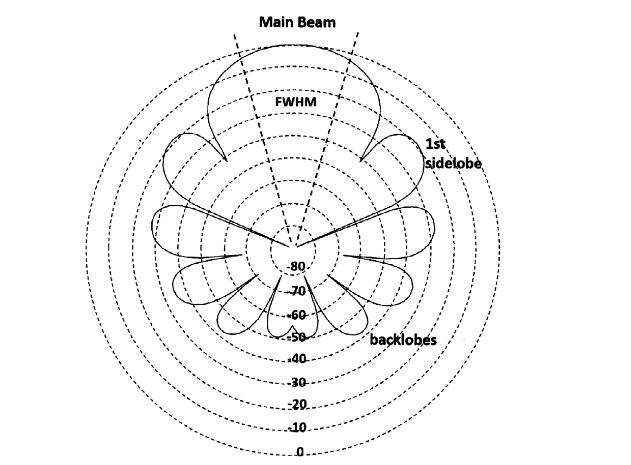
\includegraphics[scale=.65]{Figuras/largura_do_feixe.png}
\caption{Diagrama polar do padrão de radiação de uma antena, mostrando o feixe principal (\textit{main beam}), o primeiro lóbulo lateral (\textit{side lobe}) e os lóbulos traseiros (\textit{back lobes}). Fonte: \cite{burke2019introduction}.
\label{fig:Lagura_do_fexe}
}
\end{figure}

O padrão de radiação é caracterizado por uma região central de maior sensibilidade, denominada \textit{lóbulo principal}, e por estruturas secundárias chamadas \textit{lóbulos laterais}. 

\begin{itemize}
    \item O lóbulo principal determina a resolução angular do telescópio, que pode ser aproximada por \cite{cheng2009telescope_Desing}:

\begin{equation}
\theta_{\mathrm{FWHM}} \approx 1.22 \frac{\lambda}{D},
\end{equation}

onde $\lambda$ é o comprimento de onda observado e $D$ é o diâmetro da abertura da antena.

\item Os lóbulos laterais representam sensibilidade residual a direções fora do eixo principal e podem introduzir contaminações sistemáticas, como emissões da terra, emissões de outras fontes astronômicas fora do campo de interesse, Radiação difusa do fundo cósmico, etc \cite{cheng2009telescope_Desing}..
\end{itemize}

Radiotelescópio que recebe sinais muito fracos de suas radiofontes, até mesmos a radiação térmica do solo ( com temperatura próxima \(T \approx 300K\)) que são captadas pelos lóbulos secundários, acabam interferindo na relação sinal-ruido (S/R), assim como, a radiação recebida de fora da borda do refletor principal (spillover) também prejudica a recepção do sinal emitido pela radiofonte \cite{sasao2009_radioantennas}, como representa a figura \ref{fig:Lobulo principal/secundario}.

\begin{figure}[hbtp]
\centering
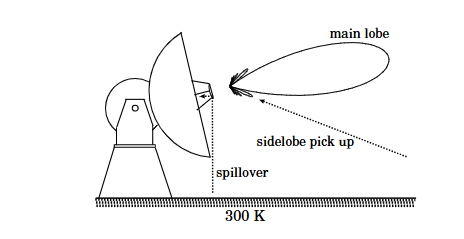
\includegraphics[scale=.8]{Figuras/lobulo_principal.png}
\caption{Representação esquemática do feixe principal, lóbulos laterais e spillover em uma antena de radiotelescópio. Fonte: \cite{sasao2009_radioantennas}.
\label{fig:Lobulo principal/secundario}
}
\end{figure}


Para um radiotelescópio \textit{single dish}, o feixe determina a resolução angular do instrumento e atua como uma função de ponderação espacial aplicada ao brilho do céu. Assim, a temperatura medida pelo detector em um dado instante pode ser expressa como a convolução entre o padrão de radiação da antena e a distribuição de temperatura de brilho do céu \cite{nikolova2025noise}:

\begin{equation}
T_A(\theta_0,\phi_0)
=
\int_{4\pi}
P_n(\theta - \theta_0,\phi - \phi_0)
\, T_B(\theta,\phi)
\, d\Omega,
\label{eq:antenna_temperature_convolution}
\end{equation}

onde $P_n(\theta - \theta_0,\phi - \phi_0)$ representa o padrão de radiação normalizado, $ T_B(\theta,\phi)$ é a temperatura de brilho do céu e $d\Omega$ é o elemento de ângulo sólido.

\subsection{Aproximação Gaussiana do Feixe}
Em muitos experimentos cosmológicos, o feixe é modelado como uma função Gaussiana bidimensional. dessa forma, é possível gerar um modelo estimado através da transformada de uma função de iluminação com taper gaussiano sobre uma abertura circular, definida por \cite{harper2018potential}: 

\begin{equation}
E(\rho) = e^{-\frac{1}{2}\left(\frac{\rho}{\sigma_b}\right)^2},
\end{equation}

onde \(\sigma\) é a largura do taper gaussiano e \(\rho\) é o número de comprimentos de onda ao longo da abertura, expresso por: 

\begin{equation}
    \rho = \frac{D}{2 \,\Lambda},
\end{equation}

sendo, \(D\)  o diâmetro da antena parabólica e \(\lambda\) o comprimento de onda.

Assumindo simetria azimutal do padrão de radiação, o feixe normalizado pode ser obtido a partir da transformada da iluminação da abertura, \cite{harper2018potential}

\begin{equation}
B_r(\theta) =
\frac{\displaystyle \int_0^{\rho_{\max}} E(\rho)\,
j_0\!\left(\rho \sin\theta\right)\,
\rho\, d\rho}
{\displaystyle \int_0^{\rho_{\max}} E(\rho)\,
\rho\, d\rho}
\label{eq:beam_pattern}
\end{equation}

o feixe é dado pela razão entre a transformada ponderada da função de iluminação e o fator de normalização correspondente, onde \(j_0\) representa a função de Bessel de primeira espécie e ordem zero.

O ganho direto do feixe é então determinado pela razão entre a área total da esfera e a integral do padrão normalizado sobre todas as co-latitudes \cite{harper2018potential}. Assim, obtém-se:

\begin{equation}
G_r =
\frac{4\pi}
{\displaystyle \int_0^{\pi}
B_r(\theta)\,
\sin\theta\, d\theta}
\label{eq:beam_gain}
\end{equation}

Aplicando esse procedimento para frequências entre 750 e 1400 MHz, os modelos resultantes apresentam ganhos típicos no intervalo \cite{harper2018potential}:

\begin{equation}
40 \ \text{dBi} \; < \; G \; < \; 46 \ \text{dBi}.
\end{equation}





%-------------------------------------------------------------------------------------------------------------------------------------------------------------------------------


\section{Backends Digitais}
Após a coleta da radiação pela antena e sua amplificação pelo sistema receptor, o sinal de rádio frequência (RF) é convertido para uma frequência intermediária (IF) e posteriormente digitalizado. O conjunto de dispositivos responsáveis pelo processamento digital desse sinal constitui o \textit{backend} do radiotelescópio. 

Os backends digitais desempenham papel fundamental na determinação da resolução espectral, largura de banda efetiva, estabilidade temporal e propriedades estatísticas do dado observado, impactando diretamente a modelagem do \textit{Time-Ordered Data} (TOD).

\subsection{Espectrômetro}

Espectrômetros digitais são instrumentos destinados a medir a distribuição espectral do sinal recebido, isto é, a potência como função da frequência \cite{wilson2013tools}. Em radioastronomia moderna, essa operação é geralmente realizada por meio de transformadas rápidas de Fourier (FFT) aplicadas ao sinal digitalizado.

O método da Transformada Rápida de Fourier (FFT) transforma o sinal temporal amostrado \(V(t)\) em sua representação no domínio da frequência \(V(\nu)\) possibilitando a estimativa do espectro de potência \(P(\nu)= \left| V(\nu) \right|^2 \) \cite{wilson2013tools}, representado na Figura \ref{fig:FFT}. De forma, que a expressão que representa como o espectro de potencia é obtido é dado, por: 

\begin{equation}
    P(\nu)= \left| \mathcal{F}\{v(t)\} \right|^2,
\end{equation}

onde $\mathcal{F}$ denota a transformada de Fourier.

\begin{figure}[hbtp]
\centering
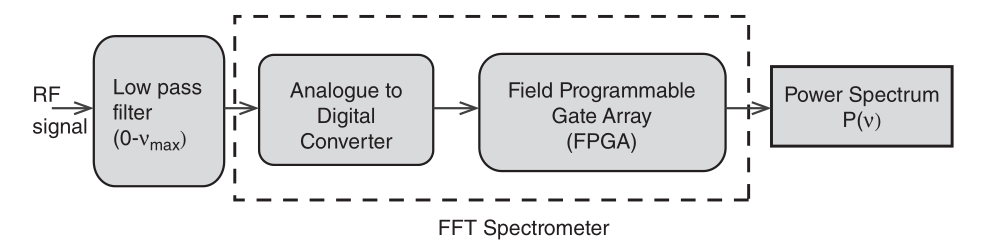
\includegraphics[scale=.5]{Figuras/FFT(1).png}
\caption{Fluxo funcional de um espectrômetro digital baseado em FFT. Fonte: \cite{burke2019introduction}.
\label{fig:FFT}
}
\end{figure}

O diagrama~\ref{fig:FFT} representa o fluxo funcional de um espectrômetro digital baseado em FFT, desde o sinal analógico recebido até a obtenção do espectro de potência\cite{burke2019introduction}. O sinal de radiofrequência (RF) proveniente do radiotelescópio é inicialmente submetido a um filtro passa-baixa, cuja função é limitar a banda observacional ao intervalo $0 \leq \nu \leq \nu_{\text{max}}$ e evitar \textit{aliasing} no processo de digitalização. 

Em seguida, o sinal filtrado é convertido para o domínio digital por meio de um conversor analógico-digital (ADC), que amostra o sinal no tempo com determinada taxa de amostragem e resolução em bits \cite{burke2019introduction}. A sequência discreta resultante é então processada em hardware digital --- tipicamente implementado em FPGA --- onde se aplica a Transformada Rápida de Fourier (FFT). 

O produto final do \textit{backend} é, portanto, a distribuição de potência em função da frequência \cite{burke2019introduction}, que constitui a base para a análise espectral e, no contexto cosmológico, para a construção de mapas em \textit{bins} de frequência associados a intervalos de \textit{redshift}.

Espectrômetros podem operar em modo de banda larga para levantamentos cosmológicos ou em alta resolução espectral para detecção de linhas estreitas \cite{burke2019introduction, wilson2013tools}, como emissões de hidrogênio neutro (HI). A estabilidade de ganho e a linearidade do backend são críticas para evitar distorções sistemáticas no espectro medido.
%------------------------------------------------------------------------------------------------------------------------------------------------------------------------------

\subsection{Correlacionadores}

Correlacionadores são sistemas analógicos ou digitais projetados para estimar funções de correlação entre sinais elétricos provenientes do receptor, com o objetivo de extrair propriedades estatísticas fisicamente relevantes do campo eletromagnético recebido. A correlação mede o grau de similaridade entre sinais como função do atraso temporal $\tau$ \cite{thompson2017interferometry}.

Em radioastronomia, correlacionadores podem operar no regime de autocorrelação ou de correlação cruzada, dependendo do número e da natureza dos sinais analisados \cite{Hagen2002}.

\begin{itemize}

\item \textbf{Correlação Cruzada:}  
A correlação cruzada envolve dois sinais distintos, sendo amplamente utilizada em experimentos interferométricos, nos quais se correlacionam sinais provenientes de diferentes antenas ou diferentes canais de polarização. Para dois sinais complexos $v_1(t)$ e $v_2(t)$, define-se \cite{Heiles2001}:

\begin{equation}
R_{12}(\tau) = \langle v_1(t)\, v_2^*(t+\tau) \rangle,
\end{equation}

onde $^*$ denota conjugação complexa e $\langle \cdot \rangle$ representa média temporal.

A função de correlação cruzada não possui simetria restrita; em geral,

\begin{equation}
R_{12}(\tau) \neq R_{12}(-\tau),
\end{equation}

o que implica que sua transformada de Fourier é, em geral, uma função complexa. A parte real e a parte imaginária dessa transformada codificam a fase relativa entre os sinais correlacionados, permitindo a determinação dos parâmetros de polarização da radiação \cite{Heiles2001, wilson2013tools}.

No contexto interferométrico, a transformada de Fourier da correlação cruzada fornece as visibilidades complexas, que representam amostras da transformada de Fourier da distribuição angular de brilho do céu \cite{thompson2017interferometry}. Essas quantidades contêm informação sobre coerência espacial e polarização da radiação.

\item \textbf{Autocorrelação:}  
Quando a correlação é realizada entre um sinal e ele mesmo, define-se a função de autocorrelação \cite{Lopez2023, Hagen2002}:

\begin{equation}
R_{xx}(\tau) = \langle v_x(t)\, v_x^*(t+\tau) \rangle.
\label{autocorrelacao}
\end{equation}

Para processos estacionários, a autocorrelação satisfaz a propriedade hermitiana

\begin{equation}
R_{xx}(\tau) = R_{xx}^*(-\tau),
\end{equation}

o que implica que sua transformada de Fourier é uma função real e não-negativa.

Pelo teorema de Wiener–Khinchin, o espectro de potência do sinal é dado pela transformada de Fourier da função de autocorrelação \cite{Hagen2002}:

\begin{equation}
P(\nu) = \int_{-\infty}^{+\infty} R_{xx}(\tau)\, e^{-2\pi i \nu \tau}\, d\tau.
\end{equation}

Como consequência, o resultado corresponde à distribuição de potência em frequência, não contendo informação de fase independente.

No regime \textit{Single Dish}, como no caso do experimento BINGO, o interesse observacional está na intensidade total do sinal recebido por cada feixe individual. Nesse contexto, o backend implementa um correlacionador de autocorrelação, no qual o sinal é correlacionado consigo mesmo para a obtenção do espectro de potência por canal de frequência.
\end{itemize}

%------------------------------------------------------------------------------------------------------------------------------------------------------------------------------
\subsection{Filtragem}

A filtragem constitui uma etapa essencial no processamento do sinal, sendo responsável por definir a banda observacional, suprimir componentes espectrais indesejadas, evitar aliasing e determinar a resolução espectral do sistema.

Os filtros podem ser classificados em duas categorias principais: analógicos e digitais. Filtros analógicos são implementados por meio de componentes eletrônicos no front-end do receptor, enquanto filtros digitais operam sobre sinais discretizados, utilizando algoritmos numéricos para modificar seu conteúdo espectral \cite{MarcelobjApostilaPDS}.

\paragraph{Filtro passa-banda}

Um filtro passa-banda permite a passagem de uma faixa específica de frequências, atenuando as componentes fora desse intervalo \cite{Pimental2022}. Em sistemas de radiofrequência, tais filtros são utilizados para selecionar a banda científica de interesse e rejeitar interferências externas.

No experimento BINGO, após a recepção e amplificação criogênica, o sinal analógico é convertido para uma frequência intermediária (IF) e submetido a um estágio de filtragem passa-banda analógica. Esse filtro define a faixa operacional do experimento, tipicamente entre aproximadamente 980–1260 MHz, correspondente ao intervalo de redshift alvo para o mapeamento da linha de 21 cm do hidrogênio neutro\cite{Wuensche2022}. Além de selecionar a banda científica, essa etapa atua como filtro anti-aliasing, prevenindo a superposição espectral decorrente da amostragem antes da digitalização \cite{MarcelobjApostilaPDS}.

\paragraph{Filtragem digital e suavização}

No domínio digital, a filtragem pode ser empregada tanto para a definição espectral via FFT quanto para suavização de mapas ou dados espectrais. Filtros Gaussianos, por exemplo, são amplamente utilizados em processamento de sinais e imagens para promover suavização controlada, atenuando componentes de alta frequência associadas ao ruído \cite{Souza2024}.

A função Gaussiana bidimensional pode ser escrita como:

\begin{equation}
    G(x,y) = \frac{1}{2\pi\sigma^{2}} \exp\left(-\frac{x^{2}+y^{2}}{2\sigma^{2}}\right),
\end{equation}

onde $x$ e $y$ representam as coordenadas espaciais em relação ao centro do filtro e $\sigma$ é o desvio padrão, parâmetro que determina sua largura efetiva. Valores maiores de $\sigma$ produzem maior suavização, pois ampliam a contribuição de vizinhos na média ponderada aplicada durante a convolução\cite{Souza2024}. A simetria radial da função implica suavização isotrópica, característica desejável na análise de mapas.

\paragraph{FFT como banco de filtros}

A Transformada Rápida de Fourier (FFT) atua, na prática, como um banco de filtros que realiza a \textit{channelização} do sinal \cite{Holzmann2019telecomunicacao}. Cada canal espectral corresponde a uma faixa de frequência de largura $\Delta \nu$, determinada pelo tempo total da janela temporal analisada. Assim, a FFT decompõe o sinal temporal amostrado em componentes espectrais discretas, definindo diretamente a resolução em frequência do espectrômetro. A largura de frequência e dada por: 

\begin{equation}
    \Delta \nu = \frac{1}{T}
\end{equation}

onde \(T\) é o tempo da janela da FFT

Como a FFT é aplicada a segmentos finitos do sinal, surgem efeitos de vazamento espectral (\textit{spectral leakage}). Para mitigar esse fenômeno, utilizam-se funções de janela (\textit{windowing}), que modificam a ponderação temporal dos dados antes da transformada, reduzindo lóbulos laterais na resposta em frequência. A escolha da janela envolve um compromisso entre resolução espectral e supressão de vazamento \cite{MarcelobjApostilaPDS}.

No contexto desta dissertação, a filtragem está diretamente associada à definição da largura dos canais espectrais e, consequentemente, à construção de mapas de intensidade em \textit{bins} de frequência, os quais correspondem a intervalos específicos de redshift da linha de 21 cm.


\subsection{Detecção}

Após os filtros temos a etapa de detecção que consiste na conversão do sinal eletromagnético oscilante, representado pelo campo elétrico $E(t)$, em uma grandeza proporcional à potência média recebida \cite{Vieira2020}. 

Em receptores do tipo total power, como no experimento BINGO, essa conversão é realizada por meio de detecção incoerente (ou \textit{square-law detection}), na qual a potência instantânea é proporcional ao quadrado do módulo do sinal \cite{burke2019introduction}:

\begin{equation}
P(t) \propto |E(t)|^2.
\end{equation}

Esse processo elimina a informação de fase do sinal, preservando apenas sua intensidade média. A potência detectada está relacionada à temperatura de antena por meio da equação radiométrica \cite{Daniyan2011, Balanis2005}

\begin{equation}
P_0 = k_B T_{\mathrm{ant}} \Delta \nu,
\label{potebcia-de-ruido}
\end{equation}

onde $k_B$ é a constante de Boltzmann e $\Delta \nu$ é a largura de banda do sistema \cite{Daniyan2011, Balanis2005}. Assim, a detecção converte flutuações do campo elétrico em estimativas de potência que serão posteriormente integradas no tempo para reduzir o ruído estatístico.



\subsection{Integração Temporal}

Após a etapa de detecção, o sinal corresponde a uma estimativa instantânea da potência recebida, ainda fortemente afetada por flutuações estatísticas associadas ao ruído térmico do sistema. A integração temporal consiste na média do sinal detectado ao longo de um intervalo de tempo $\tau$, com o objetivo de reduzir a variância da estimativa de temperatura de antena \cite{burke2019introduction}.

A sensibilidade de um radiômetro do tipo \textit{total power} é descrita pela equação do radiômetro,

\begin{equation}
\sigma_T = \frac{T_{\mathrm{sys}}}{\sqrt{\Delta \nu \, \tau}},
\label{radiometro}
\end{equation}

onde $T_{\mathrm{sys}}$ é a temperatura de sistema, $\Delta \nu$ é a largura de banda observacional e $\tau$ é o tempo de integração. Essa relação evidencia que a sensibilidade melhora proporcionalmente à raiz quadrada do produto entre largura de banda e tempo de integração \cite{Vieira2020,  burke2019introduction}.

A equação~(\ref{radiometro}) é uma das relações fundamentais da radioastronomia. Nessa expressão, $T_{\mathrm{sys}}$ representa a temperatura total do sistema, $\Delta \nu$ a largura de banda efetiva e $\tau$ o tempo de integração. A equação é exata no caso ideal de banda retangular e quando $T_{\mathrm{sys}}$ pode ser considerado uniforme ao longo da banda observacional. Fisicamente, o receptor mede a potência média $P_0 = k_B T_{\mathrm{sys}} \Delta \nu$, que, embora constante em valor médio, apresenta flutuações estatísticas decorrentes do ruído térmico \cite{burke2019introduction}.

O aumento da largura de banda eleva a potência total medida e, simultaneamente, reduz as flutuações relativas, pois o número de amostras estatisticamente independentes cresce proporcionalmente a $\Delta \nu \, \tau$. De forma análoga, a integração temporal promove a redução da variância pela média estatística, implicando que a incerteza decresce apenas com a raiz quadrada do tempo de observação. Em sistemas digitalizados, pode ser necessário incluir um fator de correção associado à quantização do sinal, dependente do número de bits por amostra. Assim, a detecção de sinais cosmológicos fracos exige necessariamente bandas largas e longos tempos de integração \cite{burke2019introduction}.


No contexto do BINGO, a integração temporal está diretamente associada à construção dos dados \textit{Time-Ordered Data} (TOD), nos quais cada amostra corresponde a uma média temporal da potência medida em um determinado canal espectral. Esses dados são posteriormente projetados em mapas, onde o tempo total de observação por pixel determina a sensibilidade final da medida cosmológica.
%-------------------------------------------------------------------------------------------------------------------------------------------------------------------------------
\section{Objetos do céu}
A modelagem do céu em radiofrequência é fundamental para experimentos de mapeamento em intensidade, pois o sinal cosmológico de interesse encontra-se imerso em múltiplos componentes astrofísicos. Nesta seção são descritas as principais contribuições espectrais relevantes na faixa observacional do BINGO.

\subsection{Linha de 21 cm do Hidrogênio Neutro}

Em 1944, Hendrik van de Hulst previu teoricamente que o hidrogênio neutro (\textit{HI}) apresentaria uma linha de emissão em um comprimento de onda específico na faixa de rádio. Com comprimento de onda de \(21{,}1\,\text{cm}\) e frequência de \(1420{,}405751\,\text{MHz}\), essa radiação ficou conhecida como linha de \(21\,\text{cm}\) \cite{ufrgs_21cm_line, hossain2018salsa}. Esse fenômeno origina-se de uma transição hiperfina do átomo de hidrogênio neutro, associada à mudança na orientação relativa dos spins (momento angular intrínseco) do elétron e do próton.

Sua frequência de repouso é dada por:

\begin{equation}
    \nu_{\mathrm{HI}} = 1420.405751 \text{ MHz}
\end{equation}

No átomo de hidrogênio neutro, tanto o elétron quanto o próton possuem spin. A interação magnética entre esses spins dá origem a dois níveis de energia ligeiramente distintos, caracterizados pela orientação relativa entre eles. Quando os spins estão alinhados paralelamente, o sistema encontra-se no estado de maior energia; quando antiparalelos, no estado de menor energia \cite{ufrgs_21cm_line}.

A transição espontânea do estado paralelo (triplete) para o antiparalelo (singlete) resulta na emissão de um fóton com comprimento de onda aproximado de \(21\,\text{cm}\). Essa transição é extremamente rara, com coeficiente de Einstein para emissão espontânea dado por \cite{EEL2018}:

\begin{equation}
A_{10} \approx 2{,}85 \times 10^{-15} \text{s}^{-1},
\end{equation}

o que corresponde a um tempo médio de vida da ordem de \(10^7\) anos para um átomo isolado. Apesar disso, devido à enorme abundância de hidrogênio neutro no meio interestelar e intergaláctico, a emissão coletiva torna-se observável \cite{ufrgs_21cm_line, hossain2018salsa}.

Atualmente, a linha de \(21\,\mathrm{cm}\) é amplamente utilizada como traçador da distribuição de matéria no Universo, sendo fundamental para estudos de mapeamento do céu em rádio. Por meio das flutuações da temperatura de brilho associadas ao hidrogênio neutro, é possível investigar a evolução da estrutura em grande escala (\textit{Large Scale Structure} – LSS) ao longo de amplos intervalos de redshift \cite{harper2018potential}. Essas flutuações permitem sondar o espectro primordial de perturbações de densidade e impor restrições às condições iniciais do Universo, bem como à natureza da matéria escura e da energia escura \cite{loeb2008possibility21}.

Uma das principais vantagens da linha de \(21\,\mathrm{cm}\) é sua capacidade de fornecer informação tridimensional do cosmos. Como a frequência observada é deslocada devido à expansão do Universo, a relação entre frequência observada e redshift é dada por:

\begin{equation}
\nu_{\mathrm{obs}} = \frac{\nu_{\mathrm{HI}}}{1+z},
\end{equation}

onde \(z\) é o redshift cosmológico. Assim, cada frequência observada corresponde a uma distância cosmológica específica, permitindo o mapeamento tridimensional da distribuição de matéria por meio da técnica de \textit{intensity mapping} \cite{pritchard2008evolution21,loeb2008possibility21}.

Dependendo das condições físicas do meio, o sinal de \(21\,\mathrm{cm}\) pode aparecer tanto em absorção quanto em emissão em relação à radiação cósmica de fundo em micro-ondas (CMB). A evolução desse sinal ao longo do tempo cósmico reflete processos fundamentais como o resfriamento do gás primordial, o surgimento das primeiras fontes luminosas e a reionização do Universo \cite{pritchard2008evolution21}.

As flutuações do sinal de \(21\,\mathrm{cm}\) contêm informações detalhadas sobre a formação da estrutura em grande escala. Em diferentes épocas, essas flutuações podem ser dominadas por variações na densidade da matéria, na fração de hidrogênio neutro ou pelos efeitos radiativos das primeiras estrelas e galáxias. Antes da formação das primeiras galáxias e após o término da reionização, espera-se que o sinal rastreie de maneira relativamente direta o campo de densidade da matéria, tornando-se uma ferramenta cosmológica particularmente poderosa \cite{pritchard2008evolution21}.

Entretanto, o sinal cosmológico de \(21\,\mathrm{cm}\) é intrinsecamente muito fraco quando comparado às emissões de foreground em rádio. A emissão síncrotron galáctica, proveniente da própria Via Láctea, é várias ordens de magnitude mais intensa que o sinal cosmológico esperado do HI. Além disso, efeitos instrumentais e interferência de radiofrequência (RFI) de origem antropogênica impõem desafios adicionais à detecção e à construção de mapas confiáveis do céu. Esses fatores exigem técnicas avançadas de calibração, modelagem instrumental e remoção de foregrounds \cite{harper2018potential}.

%------------------------------------------------------------------------------------------------------------------------------------------------------------------------------
\subsubsection*{Emissão Síncrotron}

A radiação síncrotron é produzida quando partículas carregadas relativísticas, principalmente elétrons, são aceleradas ao se moverem em trajetórias helicoidais ao redor de linhas de campo magnético. Essa aceleração centrípeta resulta na emissão de radiação altamente não térmica, que constitui o principal mecanismo de emissão em restos de supernovas, jatos relativísticos associados a buracos negros, núcleos ativos de galáxias (AGN), lóbulos de rádio de galáxias gigantes e outras regiões caracterizadas por campos magnéticos intensos e populações de elétrons energéticos \cite{slac_synchrotrons_explained,burke2019introduction}.

O espectro da emissão síncrotron, em uma faixa limitada de frequência, pode ser aproximado por uma lei de potência:

\begin{equation}
    I_\nu \propto \nu^{\alpha},
\end{equation}

onde \(I_\nu\) é a intensidade específica, \(\nu\) é a frequência e \(\alpha\) é o índice espectral. Essa dependência surge naturalmente quando a distribuição de energia dos elétrons relativísticos segue uma lei de potência do tipo \(N(E) \propto E^{-p}\), implicando um espectro de emissão também em lei de potência, com índice espectral relacionado ao expoente da distribuição energética \cite{EEL2018}.

Em radioastronomia, especialmente em baixas frequências, é usual empregar a aproximação de Rayleigh–Jeans para expressar o sinal em termos de temperatura de brilho \cite{EEL2018}. Nessa aproximação, a intensidade específica relaciona-se com a temperatura como \(I_\nu \propto \nu^2 T_b\), de modo que:

\begin{equation}
    T_b \propto \nu^\beta,
\end{equation}

em que \(\beta = \alpha - 2\) representa o índice espectral da temperatura de brilho. Assim, a temperatura de brilho da emissão síncrotron também pode ser descrita por uma lei de potência em frequência.

Observacionalmente, entretanto, verifica-se que o índice espectral não permanece estritamente constante ao longo da frequência, caracterizando o fenômeno conhecido como curvatura espectral. Essa curvatura pode ser atribuída a diferentes fatores físicos, como perdas radiativas dos elétrons relativísticos (por exemplo, perdas síncrotron e por espalhamento Compton inverso), desvios da distribuição de energia em relação a uma lei de potência pura e à superposição de múltiplas populações de elétrons ao longo da linha de visada\cite{EEL2018}.

Para modelar esse comportamento de forma mais realista, generaliza-se a dependência espectral da temperatura de brilho como:

\begin{equation}
    T_b \propto \nu^{\beta + C \log\left(\frac{\nu}{\nu_\rho}\right)},
\end{equation}

onde \(C\) é o parâmetro de curvatura espectral e \(\nu_\rho\) é a frequência pivô adotada como referência \cite{EEL2018}. Esse termo adicional permite que o índice espectral efetivo varie suavemente com a frequência, capturando desvios em relação à simples lei de potência e fornecendo uma descrição mais adequada da emissão síncrotron em análises observacionais de larga banda.

%--------------------------------------------------------------------------------------------------------------------------------------------------------------------------------
\subsubsection*{Emissão Free-Free}

A emissão free-free (bremsstrahlung térmica) resulta da interação Coulombiana entre elétrons livres e íons em meios ionizados \cite{burke2019introduction, ahmed2015_phys_eng_detection}. Esse processo ocorre quando elétrons são acelerados pelo campo elétrico de íons sem que haja captura, produzindo radiação contínua. Em radiofrequências, essa emissão é característica de plasmas ionizados com temperaturas eletrônicas típicas da ordem de \(T_e \sim 10^4\,\mathrm{K}\), como observado em regiões H\,\textsc{ii} do meio interestelar.

No regime opticamente fino, predominante em frequências de rádio, o espectro da emissão free-free pode ser aproximado por uma lei de potência relativamente plana. A intensidade específica apresenta dependência aproximada \(I_\nu \propto \nu^{-0.1}\), enquanto a temperatura de brilho segue \(T_b \propto \nu^{-2.1}\) \cite{burke2019introduction}. Essa dependência espectral é significativamente mais suave que a da emissão síncrotron, característica importante para a modelagem e separação de foregrounds em experimentos cosmológicos.

A emissividade free-free depende quadraticamente da densidade eletrônica e fracamente da temperatura, sendo proporcional a \(n_e^2 T_e^{-1/2}\) \cite{burke2019introduction}. Essa dependência implica forte correlação espacial com regiões de gás ionizado e traçadores como a emissão em H$\alpha$.

%--------------------------------------------------------------------------------------------------------------------------------------------------------------------------------
\subsubsection*{Radiação Cósmica de Fundo (CMB)}

A Radiação Cósmica de Fundo em Micro-Ondas (CMB) é a radiação remanescente do plasma primordial, desacoplada da matéria aproximadamente \(3{,}8 \times 10^5\) anos após o Big Bang. Seu espectro corresponde, com alta precisão, ao de um corpo negro com temperatura média \(T_0 = 2{,}725\,\mathrm{K}\) \cite{burke2019introduction}. Essa característica torna a CMB um dos campos de radiação mais bem caracterizados da física.

A CMB é quase isotrópica, apresentando anisotropias de temperatura, que codificam informações fundamentais sobre a geometria, composição e evolução do Universo. Observacionalmente, as grandezas de interesse são o campo de temperatura de brilho \(T(\theta,\phi)\) e seus estados de polarização \cite{burke2019introduction, selvaraj2021all}.

No contexto da radioastronomia e da simulação de céu, a CMB constitui um componente difuso de fundo com espectro térmico bem definido, cuja contribuição relativa depende da faixa de frequência considerada. Em frequências milimétricas, sua presença torna-se dominante e deve ser modelada com precisão; em bandas de rádio mais baixas, sua contribuição é subdominante frente aos foregrounds galácticos, mas ainda pode ser incluída como componente isotrópica nas simulações \cite{burke2019introduction}.

\subsection{Fontes Pontuais e Estruturas Extensas}

O céu em radiofrequência contém fontes extragalácticas discretas, como radiogaláxias e quasares, que aparecem como objetos pontuais na resolução angular típica de experimentos de \textit{Intensity Mapping}. Além disso, estruturas galácticas difusas, como regiões H\,\textsc{ii} e remanescentes de supernova, contribuem com emissão extensa espacialmente correlacionada \cite{EEL2018}.

Do ponto de vista instrumental, as fontes extragalácticas podem ser classificadas em duas categorias:

\begin{itemize}
    \item \textbf{Fontes resolvidas}: objetos com fluxo acima do limiar de detecção, que podem ser identificados individualmente e removidos ou mascarados dos mapas;
    \item \textbf{Fontes não resolvidas}: fontes fracas abaixo do limite instrumental, cuja contribuição coletiva é modelada estatisticamente como um processo de Poisson (shot noise).
\end{itemize}

A contribuição residual das fontes não resolvidas é descrita pela contagem diferencial de fontes, \( \frac{dN}{dS} \), e depende do primeiro momento da distribuição de fluxos. Assumindo um limiar \( S_{\mathrm{max}} \), fontes com \( S > S_{\mathrm{max}} \) são subtraídas, enquanto aquelas com \( S \le S_{\mathrm{max}} \) permanecem como fundo residual \cite{EEL2018}.

A temperatura de brilho associada às fontes pontuais não resolvidas em um pixel é então dada por

\begin{equation}
T_{\mathrm{ps}}(\nu,\hat{n}) =
\left( \frac{dB_\nu}{dT} \right)^{-1}
\frac{1}{\Omega_{\mathrm{pix}}}
\sum_{i=1}^{N} S_i(\nu),
\end{equation}

onde \( \Omega_{\mathrm{pix}} \) é o ângulo sólido do pixel e o fator \( dB_\nu/dT \) realiza a conversão entre intensidade específica e temperatura de brilho no regime de Rayleigh--Jeans \cite{EEL2018}.

A modelagem adequada desses diferentes componentes morfológicos é essencial para a construção de simulações realistas do céu e para a aplicação de técnicas de separação de componentes, uma vez que o sinal cosmológico do HI é tipicamente várias ordens de magnitude mais fraco do que os foregrounds galácticos.


%---------------------------------------------------------------------------------------------------------------------------------------------------------------------------------
\section{Modelagem do Radiotelescópio}

A resposta observacional de um radiotelescópio pode ser descrita a partir da equação de transferência radiativa na aproximação de campo distante. Nesse regime, a temperatura medida pela antena corresponde à integração ponderada da temperatura de brilho do céu pelo padrão de resposta angular do instrumento \cite{sasao2009_radioantennas}.

\subsection*{Temperatura de Antena}

A temperatura de antena \(T_{\mathrm{ant}}\) é definida como a média ponderada da temperatura de brilho do céu pelo padrão angular de potência da antena:

\begin{equation}
T_{\mathrm{ant}} =
\frac{
\displaystyle \int_{4\pi} P_n(\theta,\phi)\, T_B(\theta,\phi)\, d\Omega
}{
\displaystyle \int_{4\pi} P_n(\theta,\phi)\, d\Omega
}.
\label{eq:temperatura_normalizada}
\end{equation}

A equação~\ref{eq:temperatura_normalizada} corresponde à forma geral da temperatura de antena, na qual o padrão de potência não é assumido previamente normalizado.

Onde:

\begin{itemize}
    \item \(P_n(\theta,\phi)\) é o padrão de potência da antena;
    \item \(T_B(\theta,\phi)\) é a temperatura de brilho do céu;
    \item o denominador \(\displaystyle \int_{4\pi} P_n(\theta,\phi)\, d\Omega\) representa a integral do padrão sobre todo o ângulo sólido e garante a normalização adequada, assegurando que \(T_{\mathrm{ant}}\) seja uma média ponderada da temperatura de brilho \cite{sasao2009_radioantennas}.
\end{itemize}

Caso o feixe esteja previamente normalizado, isto é,

\[
\int_{4\pi} B(\theta,\phi,\nu)\, d\Omega = 1,
\]

a expressão pode ser escrita de forma simplificada como

\begin{equation}
T_{\mathrm{ant}}(\nu) =
\int_{4\pi}
T_b(\theta,\phi,\nu)\,
B(\theta,\phi,\nu)\,
d\Omega.
\label{eq:temperatura_feixe_normalizado}
\end{equation}

Essa expressão representa a integração da temperatura de brilho do céu ponderada pelo feixe instrumental. Consequentemente, o sinal observado corresponde a uma versão angularmente suavizada do campo verdadeiro, com resolução determinada pela largura a meia altura do feixe (\(\theta_{\mathrm{FWHM}}\)).

%---------------------------------------------------------------------------------------------------------------------------------------------------------------------------------------

\subsection{Modelo de Medição do Radiotelescópio \label{sec:modelo_de_medicao}}


Em um radiotelescópio, o sinal medido pelo detector está relacionado à potência eletromagnética recebida pela antena. Na teoria de radiometria, a potência detectada pode ser expressa como proporcional à temperatura equivalente do sistema. Ao incluir o ganho eletrônico do receptor, a potência medida ~\eqref{potebcia-de-ruido} pode ser escrita como

\begin{equation}
P = k_B \, G \, T_{\mathrm{sys}} \, \Delta \nu,
\label{potencia_ruido}
\end{equation}

onde \(k_B\) é a constante de Boltzmann, \(G\) representa o ganho do sistema, \(T_{\mathrm{sys}}\) é a temperatura total do sistema e \(\Delta \nu\) corresponde à largura de banda observada \cite{Price2018}.

De forma geral, o processo de medição em radioastronomia pode ser descrito por um operador linear que relaciona o sinal real do céu aos dados observados. Esse modelo pode ser escrito como

\begin{equation}
    d = \mathbf{R}s + n,
\label{modelo.linear.de.medicao}
\end{equation}

onde \(d\) representa os dados observados (por exemplo, \textit{time-ordered data}), \(s\) é o sinal verdadeiro do céu, \(\mathbf{R}\) é o operador de resposta instrumental que descreve como o instrumento projeta o céu nos dados observados, e \(n\) representa o ruído instrumental \cite{Monakhov2021}. 

No contexto de radiotelescópios do tipo \textit{single dish}, o operador instrumental inclui efeitos como o padrão de feixe da antena, o apontamento do telescópio e a resposta espectral do sistema. Assim, o dado observado pode ser interpretado como uma combinação entre o sinal do céu modulado pela resposta instrumental e as contribuições de ruído.

Para o caso específico do radiotelescópio BINGO, considerando a resposta instrumental do sistema, a saída temporal do radiotelescópio pode ser modelada como \cite{ramalho2023impactos}:

\begin{equation}
d(t,\nu) =
G(t,\nu)
\int_{4\pi}
B(\theta,\phi,\nu)\,
T_{\mathrm{sky}}(\theta,\phi,\nu)\,
d\Omega
+
n(t,\nu)
+
s_{\mathrm{sys}}(t,\nu),
\label{modelo_medicao_bingo}
\end{equation}

onde \(d(t,\nu)\) representa os dados observados (\textit{time-ordered data}), \(G(t,\nu)\) é o ganho instrumental dependente do tempo e da frequência, \(B(\theta,\phi,\nu)\) é o padrão de feixe da antena, \(T_{\mathrm{sky}}\) corresponde à temperatura de brilho do céu, \(n(t,\nu)\) representa o ruído térmico do sistema e \(s_{\mathrm{sys}}(t,\nu)\) inclui contribuições sistemáticas, como instabilidades de ganho, ruído do tipo \(1/f\) e imperfeições de calibração.

O ruído térmico \(\sigma_T\) pode ser estimado pela equação do radiômetro apresentada na equação~\eqref{radiometro}. Essa relação estabelece que a incerteza estatística associada à medição da temperatura diminui com o aumento da largura de banda observacional e do tempo de integração. Em termos físicos, isso ocorre porque o radiômetro realiza uma média temporal das flutuações aleatórias do campo eletromagnético recebido pela antena.

Em radiotelescópios do tipo \textit{single dish}, o ruído térmico constitui uma das principais fontes de incerteza nas observações e está diretamente relacionado à temperatura total do sistema \(T_{\mathrm{sys}}\), que inclui contribuições do receptor, da atmosfera e do fundo astrofísico. Assim, a equação do radiômetro fornece uma estimativa fundamental da sensibilidade instrumental, sendo amplamente utilizada na caracterização do desempenho de experimentos de radioastronomia e no planejamento de observações.


Esse modelo constitui a base para a simulação e análise de dados em experimentos de radioastronomia do tipo \textit{single dish}, sendo amplamente utilizado na construção de séries temporais de observação e na etapa posterior de reconstrução de mapas do céu.
%-----------------------------------------------------------------------------------------------------------------------------------------------------------------------------

% --------------------------------------------------------------------------------------------
% 										Capitulo 3
% --------------------------------------------------------------------------------------------

\chapter{Técnicas Experimentais}

% --------------------------------------------------------------------------------------------
% 										Se houver seção
% --------------------------------------------------------------------------------------------

\section{Nome da seção}

% --------------------------------------------------------------------------------------------
% 										Se houver subseção
% --------------------------------------------------------------------------------------------


\subsection{Nome da Subseção}




% --------------------------------------------------------------------------------------------
% 										Capitulo 4
% --------------------------------------------------------------------------------------------

\chapter{Descrição da Pipeline}

Este capítulo descreve detalhadamente a pipeline de simulação desenvolvida, incluindo decisões de design, arquitetura do software, casos de uso e exemplos de utilização

\section{Decisões de Design}

Nesta seção, discutimos as principais decisões de design tomadas durante o desenvolvimento da pipeline, incluindo a escolha de tecnologias, padrões de arquitetura e estratégias de implementação.

\subsection{Princípios Orientadores}

O desenvolvimento da pipeline de simulação foi conduzido a partir de um conjunto de princípios de engenharia de software definidos para atender às necessidades específicas do processamento de dados observacionais em radioastronomia. Simulações desse tipo frequentemente envolvem múltiplos modelos físicos, diferentes configurações instrumentais e grandes volumes de dados, exigindo uma arquitetura capaz de acomodar modificações e expansões ao longo do ciclo de desenvolvimento \cite{sharma2025karabo}.

A modularidade foi adotada como princípio central da implementação. Nessa abordagem, cada etapa do fluxo de processamento é encapsulada em componentes independentes responsáveis por tarefas específicas, como geração de mapas de entrada, simulação instrumental, produção de Time Ordered Data e reconstrução de mapas. Essa organização reduz o acoplamento entre diferentes partes do sistema e favorece a reutilização de componentes em distintos cenários de simulação  \cite{martin2008cleancode}.

A extensibilidade constituiu outro requisito fundamental. Em aplicações voltadas à radioastronomia observacional, é comum a necessidade de incorporar novos modelos de ruído, estratégias de varredura, descrições instrumentais ou métodos de reconstrução. Dessa forma, a arquitetura foi concebida para permitir a inclusão de novas funcionalidades com impacto mínimo sobre os módulos já existentes, preservando a consistência do sistema e reduzindo o custo de manutenção.

A testabilidade foi igualmente priorizada. A separação funcional entre os módulos permite que cada componente seja validado individualmente por meio de testes específicos, facilitando a identificação de inconsistências e contribuindo para a confiabilidade dos resultados produzidos pela pipeline. o que é especialmente importante em simulações científicas, onde a precisão e a robustez dos resultados são cruciais para a interpretação dos dados observacionais.

O processo de observação simuladas geralmente envolve conjuntos de dados de grandes dimensões, principalmente em longos periodos de observação. Por essa razão, a implementação buscou minimizar operações redundantes, otimizar o fluxo de dados entre os módulos e explorar estruturas computacionais adequadas para processamento em larga escala.

Por fim, buscou-se garantir um elevado nível de documentação do software. Além da utilização de convenções padronizadas de nomenclatura, foram adotadas práticas de documentação diretamente associadas aos módulos implementados, descrevendo suas funcionalidades, parâmetros de entrada e formatos de saída. Essa abordagem facilita tanto a reprodução dos experimentos quanto a utilização futura da pipeline por outros pesquisadores.

\subsection{Escolhas Tecnológicas}

A implementação da pipeline foi realizada utilizando a linguagem Python, adotando como requisito mínimo a versão 3.10. Essa escolha foi motivada pela ampla utilização da linguagem em computação científica, pois a ligunagem Python  oferece uma sintaxe clara e concisa, o que contribui para a legibilidade do código e facilita a colaboração entre pesquisadores de diferentes áreas. Além disso, a comunidade científica tem desenvolvido uma vasta gama de bibliotecas e ferramentas em Python, como NumPy, SciPy, Astropy e Healpy, que são amplamente utilizadas para processamento de dados astronômicos e análise de mapas celestes.

Entre as bibliotecas utilizadas, destacam-se:

\begin{itemize}
    \item \textbf{NumPy:} Recorreu-se como base para manipulação de arrays, operações numéricas e manipulação de eficiénte de estrutura de dados multidimensionais. Sua implementação Sua implementação otimizada para operações vetorizadas permite realizar cálculos envolvendo grandes volumes de dados com desempenho significativamente satisfatório e superior a abordagens baseadas em loops tradicionais \cite{harris2020array}.
    \item \textbf{SciPy:} Adotado para complementar as funcionalidades do NumPy, fornecendo uma ampla gama de algoritmos e rotinas para processamento de dados, otimização, integração, interpolação e processamento de sinais. A biblioteca SciPy é amplamente reconhecida por sua eficiência e confiabilidade em aplicações científicas, o que a torna uma escolha natural para a implementação de algoritmos de simulação e análise de dados em radioastronomia \cite{virtanen2020scipy}.
    \item \textbf{Astropy:} Utilizada para manipulação de coordenadas celestes, conversão de unidades, sistemas temporais e outras operações relacionadas à astronomia. A biblioteca Astropy é amplamente adotada na comunidade astronômica devido à sua robustez, flexibilidade e ampla gama de funcionalidades específicas para o processamento de dados astronômicos \cite{Astropy2022}.
    \item \textbf{Healpy} Empregada para manipulação de mapas celestes em formato HEALPix, que é um formato amplamente utilizado para representar dados astronômicos em uma esfera. A biblioteca Healpy oferece uma série de funções para criar, manipular e visualizar mapas HEALPix, facilitando a implementação de algoritmos de simulação e análise de dados em radioastronomia \cite{gorski2005healpix}.
    \item \textbf{Matplotlib:} Aplicou-se essa biblioteca para visualização de dados e resultados, permitindo a criação de gráficos, mapas e outras representações visuais dos dados simulados. A biblioteca Matplotlib é amplamente utilizada na comunidade científica para visualização de dados em Python, oferecendo uma ampla gama de opções de personalização e suporte para diferentes tipos de gráficos \cite{hunter2007matplotlib}.
\end{itemize}

Em conjunto, essas tecnologias fornecem a infraestrutura computacional necessária para a implementação dos diferentes módulos da pipeline, atendendo simultaneamente aos requisitos de desempenho, extensibilidade e reprodutibilidade definidos na seção anterior.


\subsection{Paradigmas de Programação}

A estruturação da pipeline foi conduzida utilizando conceitos de Programação Orientada a Objetos (POO), combinados com princípios de \textit{Domain-Driven Design} (DDD) e padrões de projeto amplamente empregados em engenharia de software. Essa combinação permitiu estruturar o código de forma alinhada aos requisitos científicos do problema, favorecendo a organização dos componentes, a reutilização de funcionalidades e a evolução da arquitetura ao longo do desenvolvimento.

A POO foi adotada como paradigma principal para o desenvolvimento dos módulos da pipeline, permitindo a definição de classes e objetos que encapsulam dados e comportamentos relacionados a diferentes aspectos do processo de simulação \cite{gamma1994designpatterns}. Essa abordagem facilita a modelagem de entidades complexas, como instrumentos de observação, estratégias de varredura, de ruído, etapas de processamento e algoritmos de reconstrução, permitindo que cada elemento seja tratado como uma unidade independente e bem definida dentro do sistema.

Além da organização estrutural proporcionada pela POO, foram incorporados conceitos de \textit{Domain-Driven Design} (DDD). Essa abordagem promove uma organização que reflete a realidade científica do problema. Essa abordagem favorece a clareza e a expressividade do código, facilitando a comunicação entre os desenvolvedores e os especialistas na área, além de contribuir para a manutenção e evolução da pipeline ao longo do tempo \cite{evans2003ddd}. Como resultado, os módulos da pipeline foram organizados em torno de conceitos pertencentes ao domínio da radioastronomia observacional, favorecendo a clareza da arquitetura e simplificando a manutenção do código.

Para aumentar a flexibilidade do sistema, foram empregados padrões de projeto específicos em situações recorrentes da implementação. por exemplo, o padrão \textit{Strategy} foi utilizado para encapsular diferentes algoritmos de reconstrução, permitindo que a escolha do método seja feita de forma dinâmica durante a execução da pipeline . O padrão \textit{Factory} foi adotado para criar instâncias de diferentes tipos de instrumentos ou estratégias de varredura, facilitando a extensão do sistema com novos modelos sem a necessidade de modificar o código existente. Por sua vez, o padrão \textit{Observer} foi empregado em situações que exigem comunicação entre componentes desacoplados, permitindo que modificações de estado em determinados módulos sejam automaticamente propagadas para elementos dependentes \cite{gamma1994designpatterns}.

Em conjunto, esses paradigmas e padrões de projeto fornecem a base arquitetural que sustenta a implementação da pipeline, permitindo que sua estrutura permaneça compatível com os requisitos de extensibilidade, manutenção e evolução científica estabelecidos para o projeto.

\section{Modelagem \label{sec.modelagem}}
  


\subsection{Diagrama de Classes Geral}

A arquitetura da pipeline foi modelada utilizando os princípios da Programação Orientada a Objetos, permitindo representar os diferentes elementos do processo observacional por meio de entidades computacionais bem definidas. Essa abordagem favorece a separação de responsabilidades entre os componentes do sistema e facilita a expansão da pipeline para novos cenários de simulação.

\begin{figure}[hbtp]
    \centering
    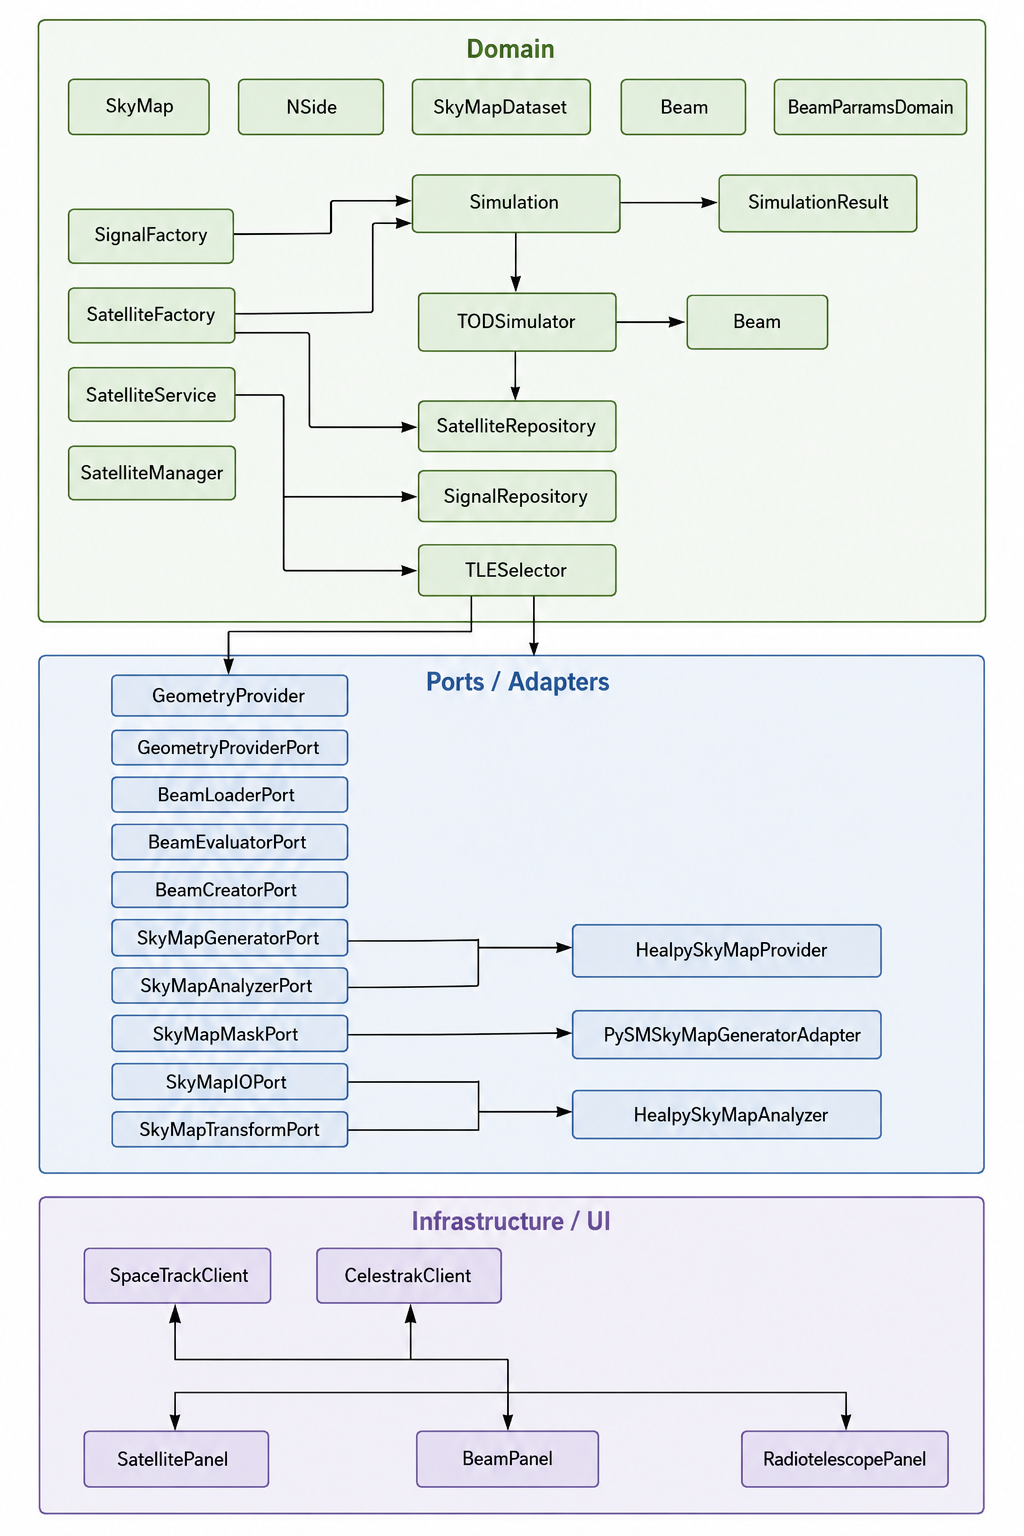
\includegraphics[scale=.4]{Figuras/diagrama_classe_pipeline0.png}
    \caption{Diagrama de classes geral da pipeline de simulação. Fonte: Elaborado pelo autor.}
    \label{fig:diagrama-classes-pipeline}
\end{figure}

A Figura~\ref{fig:diagrama-classes-pipeline} apresenta o diagrama de classes geral da pipeline, destacando as principais entidades e suas relações. O diagrama é organizado em camadas, refletindo a estrutura hierárquica do sistema e a separação de responsabilidades entre os diferentes módulos.

A camada de domínio concentra os elementos centrais da modelagem científica. Nela encontram-se classes como \texttt{SkyMap}, que representa os mapas de entrada utilizados nas simulações, \texttt{Beam} responsável por modelar a resposta instrumental e \texttt{simulation} que encapsula os parâmetros necessários para execução de um experimento observacional. A classe \texttt{simulation} atua como elemento agregador dos diferentes componentes envolvidos na execução da pipeline. Por meio dela são coordenadas as etapas de construção dos sinais simulados, obtenção da geometria observacional e geração dos dados ordenados no tempo.

Fazem parte também dessa camada os componentes relacionados à geração de sinais, simulação de dados temporais e gerenciamento de satélites, representados pelas classes:  \texttt{SignalFactory}, responsável por construir os sinais utilizados durante a simulação a partir dos modelos disponíveis nos repositórios científicos. De forma complementar, a classe \texttt{TODSimulator} aplica os efeitos instrumentais e produz as séries temporais correspondentes às observações simuladas. Para o tratamento de dados e informações orbitais, foram implementados as classes \texttt{SatelliteFactory}, \texttt{SatelliteService} e \texttt{SatelliteRepository}, responsáveis pela obtenção, armazenamento e gerenciamento de elementos orbitais utilizados para determinação da geometria observacional e análise de interferências provenientes de satélites artificiais.

A integração entre o domínio científico e as ferramentas externas é realizada por meio de um conjunto de portas (\textit{ports}) e adaptadores (\textit{adapters}). As portas definem as interfaces de comunicação entre os módulos internos da pipeline e as bibliotecas externas utilizadas para processamento de dados, manipulação de mapas celestes e visualização. Os adaptadores, por sua vez, implementam essas interfaces, possibilitando que a pipeline interaja com as bibliotecas de forma transparente, facilitando a substituição ou atualização das dependências externas sem impactar a estrutura interna do sistema.

Entre os adaptadores implementados destacam-se os componentes baseados nas bibliotecas Healpy e PySM, responsáveis pela geração, análise e manipulação de mapas celestes discretizados segundo a pixelização HEALPix. A utilização desses adaptadores garante interoperabilidade com ferramentas amplamente utilizadas na comunidade astronômica.

Por fim, a camada de infraestrutura reune os componentes destinados à aquisição de dados externos e às interfaces de interação com o usuário. Nessa categoria encontram-se os clientes responsáveis pela obtenção de dados orbitais a partir de serviços externos, bem como os painéis utilizados para configuração dos parâmetros observacionais e instrumentais.

A estrutura apresentada estabelece uma separação clara entre domínio científico, serviços de aplicação, mecanismos de integração e infraestrutura. Como resultado, a arquitetura da pipeline é capaz de acomodar a evolução científica e tecnológica ao longo do tempo, permitindo a inclusão de novos modelos, algoritmos e ferramentas sem comprometer a integridade do sistema ou a reprodutibilidade dos experimentos realizados.

\subsection{Domínios Principais}

A arquitetura da pipeline foi estruturada em torno de um conjunto de domínios especializados, cada um responsável por representar uma parte específica do processo de simulação observacional. Essa organização permite separar conceitos científicos, modelos instrumentais e mecanismos computacionais, reduzindo o acoplamento entre componentes e facilitando a evolução independente de diferentes módulos do sistema.

Os domínios implementados refletem os principais elementos envolvidos na cadeia de aquisição e processamento de dados radioastronômicos, ilustrados na Figura~\ref{fig:diagrama-pipeline-dominios}.

\begin{figure}[hbtp]
    \centering
    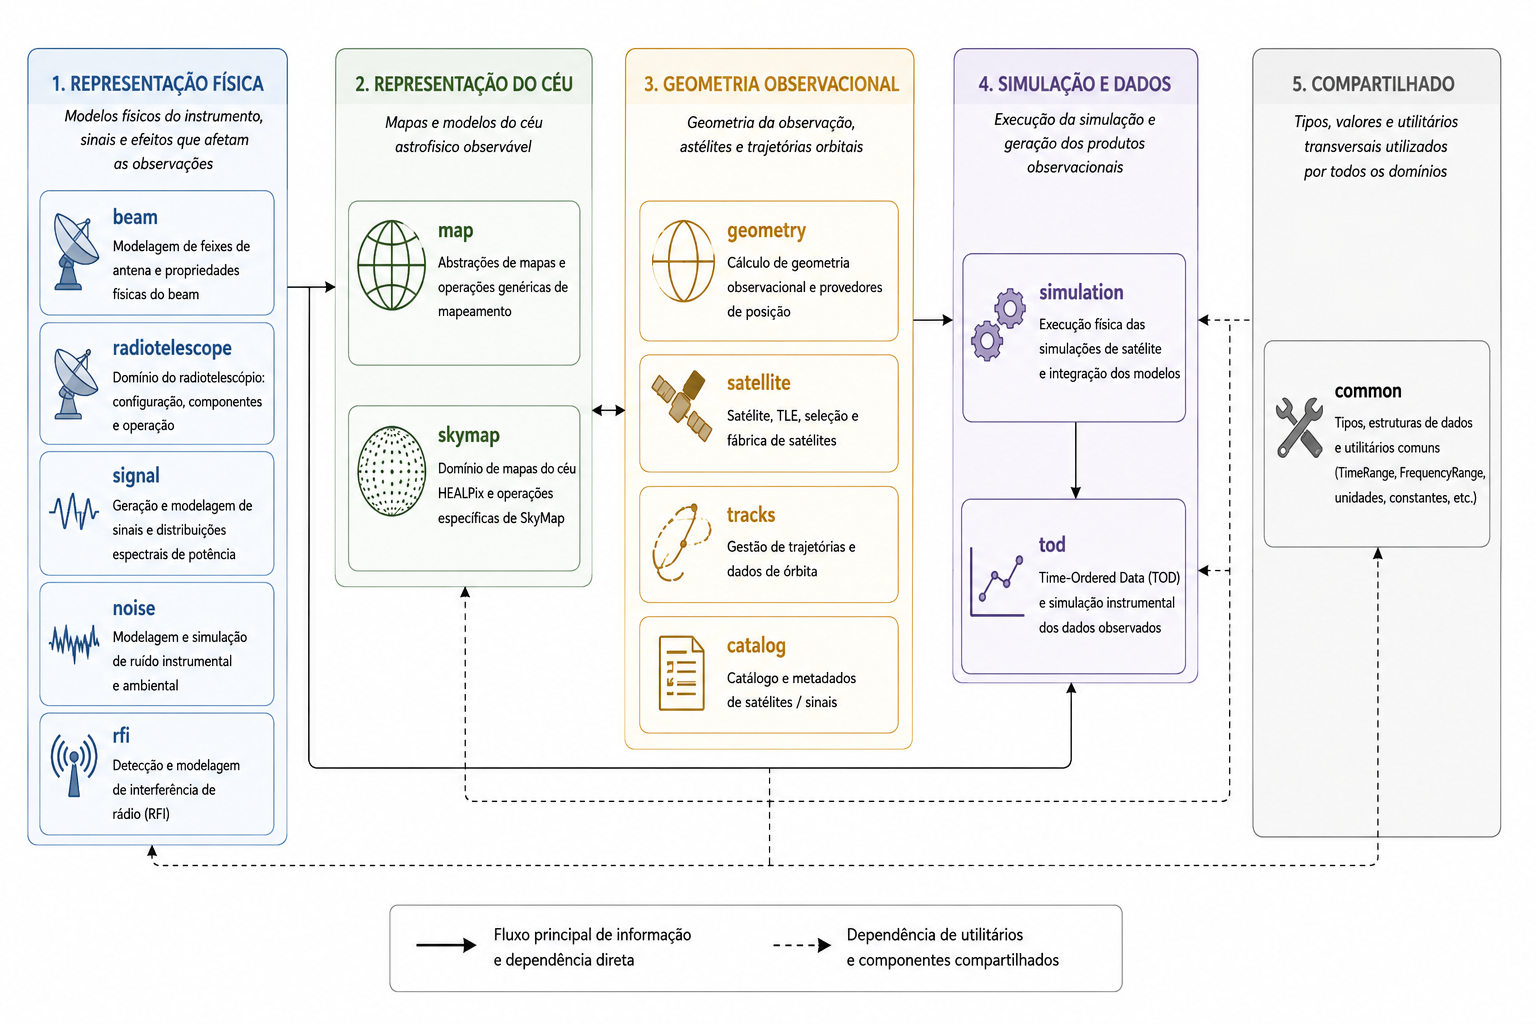
\includegraphics[scale=.32]{Figuras/dominio_pipeline.png}
    \caption{Principais domínios da pipeline de simulação. Fonte: Elaborado pelo autor.}
    \label{fig:diagrama-pipeline-dominios}
\end{figure}

\subsubsection{Domínios de Representação Física}

O domínio de representação física concentra os modelos associados ao instrumento observacional e aos processos físicos que afetam os sinais adquiridos, incluindo a resposta do feixe, a modelagem dos sinais de interesse, os mecanismos de ruído e as fontes de interferência por radiofrequência.. Ele inclui classes como \texttt{beam}, \texttt{radiotelescope}, \texttt{signal}, \texttt{noise} e \texttt{rfi}.

O domínio \texttt{beam} concentra os aspectos relacionados à resposta angular da antena, incluindo parâmetros fisicos e operações aplicadas para modelar o efeito do feixe instrumental sobre os sinais observados. O domínio \texttt{radiotelescope} representa o conjunto de características físicas e operacionais do instrumento de observação, Abrangendo a geometria da antena, a configuração de varredura e os parâmentros de aquisição de dados. 

A modelagem dos sinais observados é realizada por meio do domínio \texttt{signal}, o qual representa os diferentes componentes do sinal, como o sinal astronômico e pela descrição de distribuições espectrais de potência. Complementarmente, o domínio \texttt{noise} tem como missão, modelar os diferentes tipos de ruído presentes nas observações, assim como ruído térmico, ruído de fundo e outras fontes de interferência. O domínio \texttt{rfi} é dedicado à representação de interferências provenientes de fontes artificiais, como satélites e emissões terrestres, permitindo a modelagem de seus efeitos sobre os dados observacionais simulados.

De forma integrada, os dominios de representação física fornecem a base para a construção dos sinais simulados, a aplicação dos efeitos instrumentais e a geração dos dados ordenados no tempo, permitindo que a pipeline produza resultados realistas e cientificamente relevantes para o estudo de fenômenos astronômicos.

\subsubsection{Domínios de Representação do Céu}

A representação do céu observacional é organizada por meio dos domínios \texttt{map} e \texttt{skymap}. Esses módulos são encarregados por armazenar, manipular e processar os mapas de entrada utilizados nas simulações.

O \texttt{map} é focado em definir a estrutura de dados para representação de mapas celestes, abrangendo a definição de atributos como resolução angular, sistema de coordenadas e formato de armazenamento. Por sua vez, o domínio \texttt{skymap} implementa funcionalidades específicas para mapas HEALPix, incluindo mecanismos de acesso aos dados, aplicação de máscaras e manipulação de componentes astrofísicos.
\subsubsection{Domínios Observacionais}

A determinação da geometria observacional e do movimento dos objetos simulados é tratada pelos domínios \texttt{geometry}, \texttt{satellite}, \texttt{tracks} e \texttt{catalog}.

O domínio \texttt{geometry} modela a geometria da observação, como a posição do observador, a orientação do instrumento e a trajetória de varredura. Ele fornece métodos para calcular as coordenadas de observação. O  \texttt{satellite} concentrar as identidades associadas aos satélites artificiais, seus parâmetros orbitais, características de emissão e efeitos de interferência sobre os dados observacionais.

Complementarmente, os domínios \texttt{tracks} e \texttt{catalog} são responsáveis pelo gerenciamento de trajetórias, efemérides e metadados associados aos objetos observados. O domínio \texttt{tracks} assegura o armazenamento e processamento das trajetórias dos objetos simulados, como também, a determinação de suas posições ao longo do tempo e a análise de suas interações com o instrumento de observação. O domínio \texttt{catalog} fornece informações descritivas, classificações, identificadores e demais metadados utilizados durante as simulações.

\subsubsection{Domínios de Simulação e Produtos de Dados}

A execução das simulações e a geração dos produtos observacionais são realizadas pelos domínios \texttt{simulation} e \texttt{tod}.

O domínio \texttt{simulation} atua como elemento central da pipeline, coordenando a execução das diferentes etapas do processo de simulação. Ele fica a cargo de integrar os componentes relacionados à representação física, geometria observacional e manipulação de mapas, garantindo que as simulações sejam conduzidas de forma consistente e alinhada aos requisitos científicos estabelecidos.

Já o domínio \texttt{tod} é encarregado de representar os dados ordenados no tempo produzidos durante as simulações. Ele define a estrutura de dados para armazenar as séries temporais correspondentes às observações simuladas, informações sobre os pontos de amostragem, os valores dos sinais observados e os metadados associados. Esse domínio também implementa métodos para manipular e processar os dados temporais, facilitando a análise e interpretação dos resultados produzidos pela pipeline.

\subsubsection{Domínios Compartilhados}

Por fim, o domínio \texttt{common} reúne os elementos compartilhados entre os diferentes módulos da pipeline, incluindo classes utilitárias, funções de apoio e estruturas de dados comuns. Ele serve como um repositório central para componentes que são utilizados por múltiplos domínios, promovendo a reutilização de código e a consistência em toda a implementação da pipeline. 

A centralização desses componentes reduz redundâncias e contribui para a consistência das interfaces utilizadas pelos diferentes domínios. Essa divisão clara entre domínios especializados e elementos compartilhados favorece a organização do código, facilita a manutenção e promove a evolução independente dos diferentes módulos da pipeline ao longo do tempo. Essa organização constitui a base conceitual da arquitetura implementada e fornece os mecanismos necessários para a construção de cenários observacionais complexos de forma modular e extensível, em consonância com os princípios de modelagem orientada a domínios propostos por \citeonline{evans2003ddd}.

\subsection{Fluxo de Dados}

O fluxo de dados da pipeline foi projetado para integrar informações provenientes de múltiplas fontes e transformá-las em produtos observacionais simulados de forma estruturada e reprodutível. A Figura~\ref{fig:fluxo-dados-pipeline} apresenta uma visão geral desse processo, evidenciando as diferentes camadas da arquitetura e as interações estabelecidas entre seus componentes.

\begin{figure}[hbtp]
    \centering
    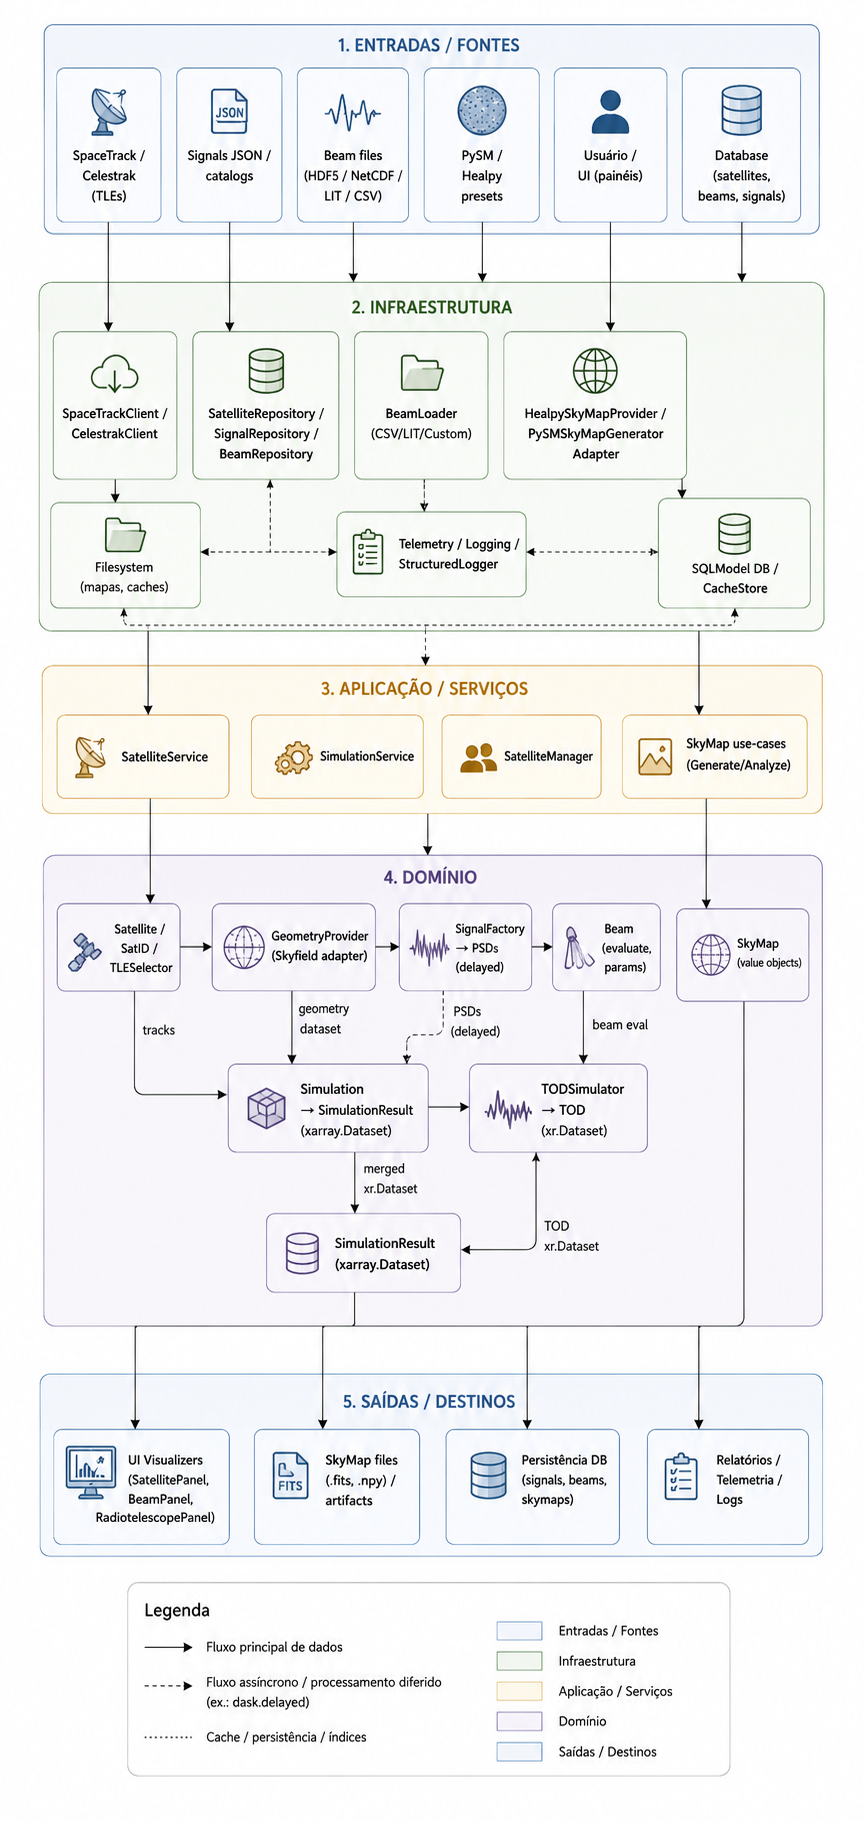
\includegraphics[scale=.38]{Figuras/Fluxo_de_dados.png}
    \caption{Fluxo de dados da pipeline de simulação. Fonte: Elaborado pelo autor.}
    \label{fig:fluxo-dados-pipeline}
\end{figure}

O processo tem início na etapa de aquisição dos dados de entrada, que inclui elementos orbitais de satélites, catálogos de sinais, modelos do feixe instrumental, mapas do céu e parâmetros fornecidos pelo usuário. Esses dados são obtidos por meio de serviços externos, repositórios científicos e interfaces de configuração, sendo processados e organizados para uso nos estagios subsequentes da pipeline.

Após a aquisição, os dados são processados pela camada de infraestrutura, responsavel pela comunicação com serviços externos, gerenciamento de arquivos e persistência das informações. Nessa etapa, os diferentes formatos de entrada são convertidos para representações compatíveis com os modelos utilizados pela pipeline, assegurando a consistência dos dados e propiciando sua manipulação nos processos seguintes. Além disso, mecanismos de armazenamento temporário e cache são empregados para otimizar o acesso aos dados e reduzir a latência durante a execução das simulações.

A camada de aplicação atua como intermediária entre os componentes de infraestrutura e os modelos científicos do domínio. Seus serviços coordenam operações relacionadas à obtenção de satélites, geração de mapas do céu e execução das simulações, encapsulando regras de negócio e certificando a integridade dos processos. Essa camada é responsável por orquestrar as interações entre os diferentes módulos, assegurando que as etapas de processamento sejam conduzidas de forma consistente e alinhada aos requisitos científicos estabelecidos para o projeto.

No núcleo da arquitetura encontram-se os modelos científicos responsáveis pela representação dos satélites, da geometria observacional, dos sinais simulados, dos mapas do céu e da resposta instrumental.  Nessa etapa, os elementos orbitais são convertidos em trajetórias observacionais, os modelos geométricos determinam a posição relativa entre o instrumento e os objetos simulados, e os sinais são gerados a partir dos modelos físicos definidos para cada cenário. Essas informações são então combinadas para produzir os dados observacionais sintéticos.

O domínio de simulação coordena a aplicação dos efeitos instrumentais sobre os sinais gerados, levando em consideração a geometria da observação e as características do feixe. O resultado desse processo é a produção dos dados ordenados no tempo (\textit{Time Ordered Data} -- TOD), que representam as séries temporais correspondentes às observações simuladas.

Os produtos gerados pela pipeline podem ser direcionados para diferentes destinos. Entre eles destacam-se as interfaces de visualização, os arquivos científicos utilizados em análises posteriores, os bancos de dados destinados à persistência dos resultados e os sistemas de telemetria empregados para monitoramento e rastreabilidade das execuções. Essa flexibilidade permite que os mesmos dados sejam utilizados em diferentes etapas do ciclo de desenvolvimento, validação e análise científica.

Além disso, a organização adotada estabelece uma separação clara entre aquisição de dados, processamento científico e geração de produtos observacionais. Essa estrutura reduz o acoplamento entre os componentes da arquitetura e permite a evolução independente dos diferentes módulos da pipeline. Como resultado, novas fontes de dados, modelos físicos e estratégias de simulação podem ser incorporados sem alterações significativas nos demais componentes do sistema, preservando a consistência da implementação e a reprodutibilidade dos experimentos realizados \cite{evans2003ddd, martin2008cleancode}.

\section{Casos de Uso}
 
Nesta seção, são apresentados casos de uso exemplares que ilustram a aplicação da pipeline de simulação em cenários específicos de interesse científico. Cada caso de uso descreve o contexto, os objetivos, os passos envolvidos na execução da simulação e os resultados esperados, demonstrando a flexibilidade e a capacidade da pipeline para atender a diferentes necessidades de pesquisa em radioastronomia observacional.

\subsection{Geração de Mapas do Céu Sintéticos}

A geração de mapas do céu sintéticos é um caso de uso fundamental da pipeline, uma vez que  que fornece a representação espacial dos sinais astronômicos simulados, servindo como base para a construção dos dados observacionais \cite{delabrouille2013psm, thorne2017pysm}. Esses mapas descrevem a distribuição da intensidade do sinal celeste sobre a esfera celeste, discretizada segundo a pixelização HEALPix \cite{gorski2005healpix}, permitindo sua utilização em estudos de observação simulada, reconstrução de mapas e análise de efeitos instrumentais.

Para atender a essa necessidade, foi desenvolvido o caso de uso \texttt{GenerateSkyMapUseCase}, responsável por coordenar o processo de criação de mapas sintéticos a partir dos parâmetros definidos. Sua implementação está localizada na camada de aplicação da arquitetura e segue os princípios de separação de responsabilidades adotados ao longo do projeto.

O processo de geração de mapas inicia-se com a definição dos parâmetros de entrada, que incluem parâmetro $N_{\mathrm{side}}$, a frequência de observação e a lista de componentes físicos que devem compor o sinal simulado. Esses parâmetros são fornecidos por meio de uma interface de configuração, permitindo que o usuário personalize a simulação de acordo com suas necessidades específicas. O parâmetro $N_{\mathrm{side}}$ determina a resolução angular do mapa HEALPix, enquanto a frequência de observação influencia a modelagem dos sinais astronômicos e dos efeitos instrumentais.

Antes de iniciar a criação do mapa, o caso de uso realiza uma validação dos parâmetros de entrada, assegurando que estejam dentro dos limites aceitáveis e que sejam consistentes com os modelos físicos disponiveis na pipeline. A frequência de observação deve assumir valores positivos e ao menos um componente físico deve ser especificado para a construção do mapa. Caso os parâmetros sejam considerados inválidos, o processo é interrompido e uma mensagem de erro é retornada ao usuário, indicando a natureza da inconsistência detectada.

Após a validação, o caso de uso converte o valor informado para um objeto de domínio do tipo \texttt{NSide}, que encapsula propriedades relacionadas à resolução angular do mapa HEALPix. Em seguida, a geração do mapa é delegada à interface \texttt{SkyMapGeneratorPort}, que define o contrato utilizado para comunicação entre a camada de aplicação e os mecanismos concretos de geração implementados na infraestrutura.

Como resultado, é produzido um objeto contendo os dados do mapa gerado, o número total de pixels e a resolução utilizada. Essas informações são encapsuladas em um objeto de transferência de dados (\textit{Data Transfer Object} -- DTO) \cite{evans2003ddd}, permitindo que os resultados sejam consumidos por outros componentes da pipeline sem dependência direta das implementações internas do processo de geração.

O Código~\ref{lst:generate-skymap} apresenta uma versão simplificada do fluxo de execução do caso de uso.

\begin{lstlisting}[
language=Python,
caption={Trecho simplificado do caso de uso de geração de mapas sintéticos.},
label={lst:generate-skymap}
]
def execute(input_dto):

    nside = NSide(input_dto.nside)

    sky_map = generator.generate(
        nside=nside,
        freq_ghz=input_dto.frequency_ghz,
        components=input_dto.components,
    )

    return GenerateSkyMapOutputDTO(
        nside=nside.value,
        npix=sky_map.npix,
        map_data=sky_map.data,
    )
\end{lstlisting}

A separação entre validação, coordenação da execução e geração física do mapa permite que diferentes mecanismos de construção de mapas sejam incorporados à pipeline sem alterações na lógica de aplicação. Dessa forma, novos modelos astrofísicos ou bibliotecas especializadas podem ser integrados por meio da implementação da interface \texttt{SkyMapGeneratorPort}, preservando a estabilidade da arquitetura e favorecendo sua extensibilidade.

\subsection{Análise de Mapas do Céu}

Após a aquisição de mapas do céu, é necessário realizar análises para extrair informações quantitativas sobre os sinais simulados. Geralmente, em estudos radioastronômicos, uma abordagem amplamente utilizada consiste na decomposição do mapa em harmônicos esféricos e na análise do espectro de potência angular associado \cite{gorski2005healpix}. O espectro angular $(C_\ell)$ fornece uma medida da distribuição de potência em diferentes escalas angulares do sinal observado, constituindo uma ferramenta fundamental para caracterização de estruturas presentes nos mapas celestes.

Com esse objetivo, a pipeline implementa o caso de uso \texttt{AnalyzeSkyMapUseCase}, responsável por coordenar a análise espectral de mapas representados pelo objeto de domínio \texttt{SkyMap}. Sua implementação segue a mesma filosofia arquitetural adotada nos demais casos de uso defendida por Evans \cite{evans2003ddd} e Martin \cite{martin2008cleancode}, concentrando-se na validação dos parâmetros de entrada e na orquestração da execução da análise.

A execução se inicia com o recebimento de um objeto contendo o mapa a ser analisado e, opcionalmente, o valor máximo do multipolo angular $(\ell_{\mathrm{max}})$. A priori, são realizadas verificações para assegurar que o mapa fornecido seja válido e compativel com a estruttura de dados utilizada pela pipeline. O mapa deve conter um número de pixels consistente com a resolução angular definida pelo parâmetro $N_{\mathrm{side}}$, e os dados devem estar organizados de acordo com o formato HEALPix.

Em seguida, o caso de uso delega o calculo do espectro de potência angular à interface \texttt{SkyMapAnalyzerPort}, que define o contrato para comunicação entre a camada de aplicação e os mecanismos concretos de análise implementados na infraestrutura. O resultado desse processo é um objeto contendo os valores do espectro de potência angular para cada multipolo até o valor máximo especificado. Esses resultados são encapsulados em um DTO, permitindo que sejam consumidos por outros componentes da pipeline para análises posteriores ou visualização.

O Código~\ref{lst} apresenta um trecho simplificado da execução desse caso de uso.

\begin{lstlisting}[
language=Python,
caption={Trecho simplificado do caso de uso de análise de mapas do céu.},
label={lst}
]
cls = self._analyzer.compute_cls(
skymap=sky_map,
lmax=input_dto.lmax,
)

return AnalyzeSkyMapOutputDTO(
nside=sky_map.nside_value,
lmax=input_dto.lmax,
cls=cls,
)
\end{lstlisting}

Observa-se que a separação entre validação, coordenação da execução e análise física do mapa permite que diferentes algoritmos de análise sejam incorporados à pipeline sem alterações na lógica de aplicação. Além disso, esse caso de uso pode ser empregado na análise de mapas provenientes de observações reais ou de outras ferramentas de simulação.



\section{Estrutura do Código}

A implementação da pipeline de simulação foi organizada em uma estrutura de código modular, seguindo os princípios de engenharia de software e as melhores práticas de desenvolvimento. A estrutura adotada reflete a arquitetura definida para o sistema, facilitando a manutenção, evolução e colaboração entre os desenvolvedores.

\subsection{Organização de Diretórios}

A organização do código-fonte foi concebida para refletir diretamente a arquitetura apresentada nas seções anteriores, adotando princípios de separação de responsabilidades, baixo acoplamento e independência entre domínios científicos e componentes tecnológicos. A estrutura do projeto segue uma divisão em camadas, permitindo que os modelos científicos permaneçam desacoplados dos mecanismos de persistência, interfaces de usuário e bibliotecas externas. A estrutura de diretórios é organizada da seguinte forma: 

A Figura~\ref{fig:estrutura-codigo} apresenta uma visão resumida da organização dos principais diretórios do projeto.

\begin{figure}[hbtp]
    \centering
    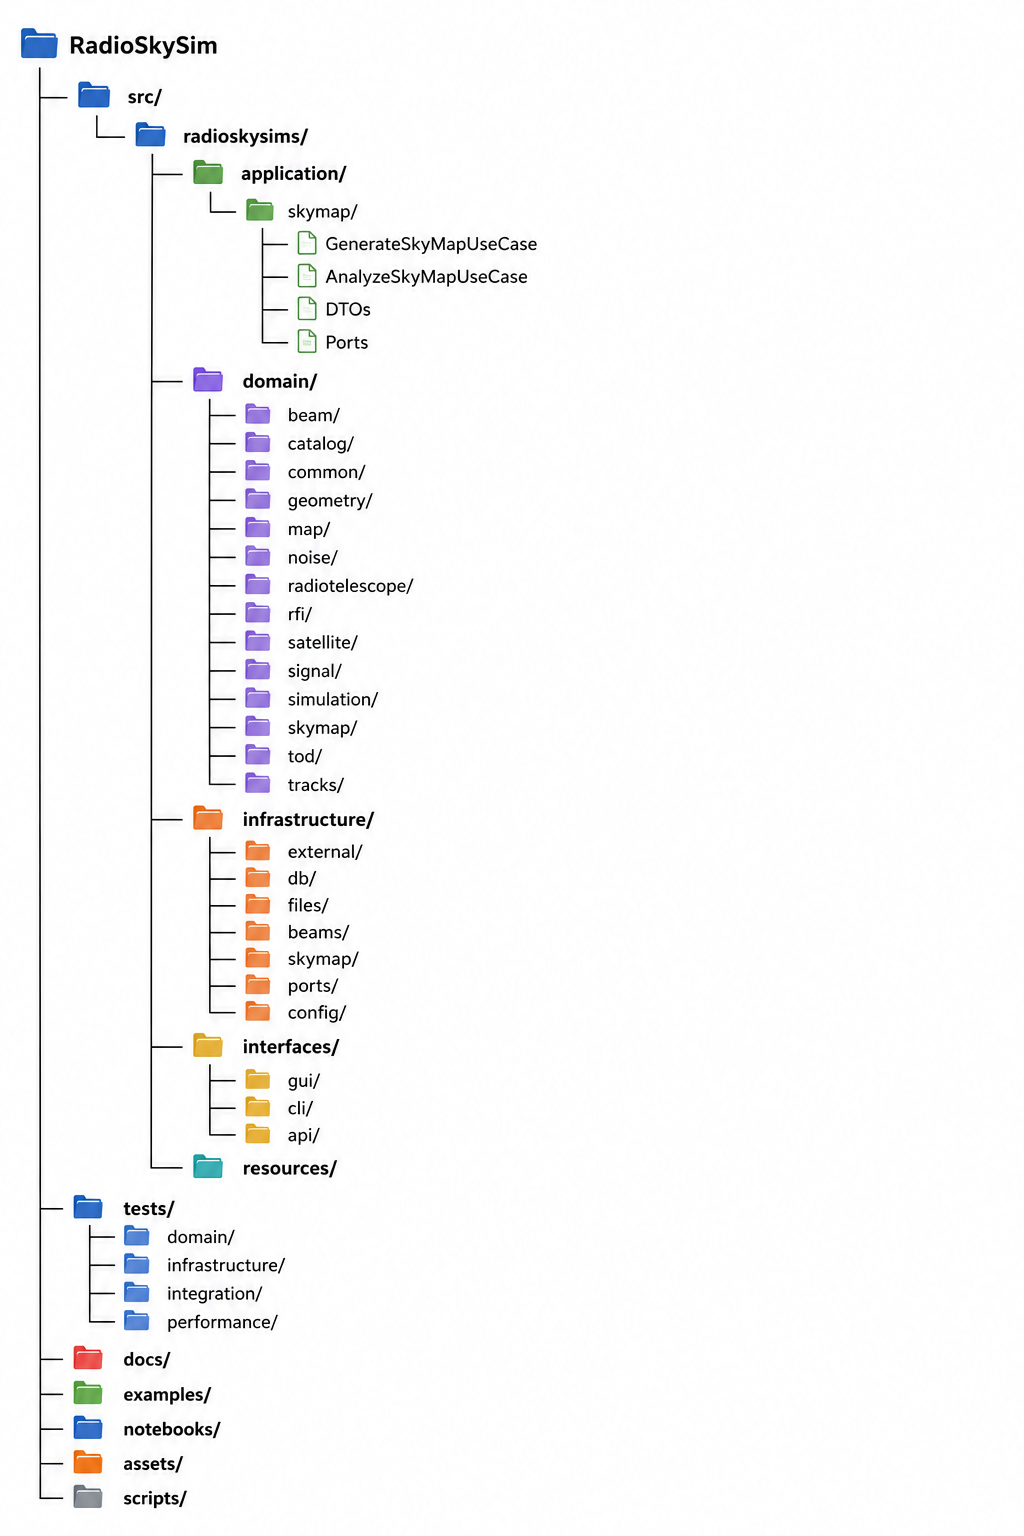
\includegraphics[scale=.4]{Figuras/Organização_diretorio.png}
    \caption{Estrutura de diretórios do código-fonte da pipeline de simulação. Fonte: Elaborado pelo autor.}
    \label{fig:estrutura-codigo}
\end{figure}

Os componentes centrais da aplicação estão localizados no diretório \texttt{src/radioskysims}, que concentra a implementação da pipeline científica. Sua organização segue uma divisão em quatro grupos principais: aplicação, domínio, infraestrutura e interfaces.

O diretório \texttt{domain} reúne os modelos científicos e conceitos fundamentais utilizados pela pipeline. Nessa camada encontram-se os domínios responsáveis pela modelagem do céu, instrumentação, sinais, ruídos, satélites, geometria observacional e dados ordenados no tempo. A organização interna desse diretório reflete a divisão em domínios apresentada na seção de modelagem \ref{sec.modelagem}, permitindo que cada módulo seja desenvolvido e mantido de forma independente, favorecendo a evolução científica da pipeline ao longo do tempo.

A camada de aplicação, localizada no diretório \texttt{application}. Tem como missão coordenar a execução dos casos de uso, realizar validações de entrada e orquestrar as interações entre os diferentes domínios científicos e os mecanismos de infraestrutura. Os casos de uso de geração e análise de mapas do céu apresentados anteriormente são exemplos de funcionalidades implementadas nessa camada.

Os componentes responsáveis pela comunicação com sistemas externos encontram-se no diretório \texttt{infrastructure}, que inclui implementações de repositórios, adaptadores para serviços externos, mecanismos de persistência, carregamento de arquivos científicos e implementações concretas das portas utilizadas pela aplicação.

As interfaces que é disponibilizadas para interação com o usuário são organizadas no diretório \texttt{interfaces}. Nesse modulo estão incluido  aplicações gráficas, interfaces de linha de comando e possíveis serviços de API.

Complementando a estrutura principal, o diretório \texttt{tests} reúne testes unitários, testes de integração e avaliações de desempenho. Essa organização favorece a validação sistemática dos componentes implementados e contribui para a confiabilidade dos resultados produzidos pela pipeline.

\subsection{Módulos Principais}

A implementação da pipeline foi organizada em módulos especializados, cada um responsável por uma parcela específica da modelagem científica. Os módulos principais da aplicação correspondem aos elementos fundamentais envolvidos na geração dos dados observacionais simulados, abrangendo desde a representação do céu até a produção dos dados ordenados no tempo e dos produtos finais da simulação.


\subsubsection{Módulo SkyMap}

O módulo \texttt{skymap} é responsável pela representação dos mapas do céu utilizados pela pipeline. Sua implementação baseia-se na pixelização HEALPix, amplamente empregada em aplicações astronômicas devido à sua capacidade de representar dados sobre a esfera com resolução uniforme \cite{gorski2005healpix}.

Além do armazenamento dos mapas, esse módulo fornece operações para leitura, escrita, mascaramento, transformação e análise de dados observacionais. Os objetos definidos nesse domínio constituem a principal interface entre os modelos astrofísicos de entrada e os processos de simulação observacional.

\subsubsection{Módulo Beam}

O \texttt{beam} concentra a modelagem da resposta angular do instrumento. Ele define estruturas responsáveis por representar padrões de feixe, parâmetros instrumentais e métodos de avaliação da resposta da antena em diferentes direções do céu.

A modelagem do feixe desempenha papel fundamental na simulação observacional, pois determina como a distribuição de brilho celeste é convoluída pela resposta espacial do instrumento durante o processo de aquisição dos dados.

\subsubsection{Módulo Satellite}

 A representação dos satélites artificiais considerados nas simulações fica a cargo do \texttt{satellite}. Ele reúne entidades associadas aos elementos orbitais, identificadores NORAD, seleção de satélites e construção de cenários observacionais envolvendo diferentes constelações.

Esse módulo atua em conjunto com os componentes de geometria observacional para determinar a posição aparente dos satélites ao longo do tempo e avaliar sua contribuição para os sinais simulados.

\subsubsection{Módulo Geometry}

O \texttt{geometry} implementa os cálculos necessários para determinar a geometria observacional entre o radiotelescópio e os objetos simulados. Suas funcionalidades incluem o cálculo de azimute, elevação, distância e demais parâmetros geométricos utilizados durante a geração dos sinais observacionais.

Os resultados produzidos por esse módulo servem como entrada para os processos de modelagem instrumental e geração dos dados ordenados no tempo.

\subsubsection{Módulo Signal}

Quem se encarregar pela modelagem dos sinais eletromagnéticos que são considerados na simulação é o \texttt{signal}. Ele define mecanismos para geração de distribuições espectrais de potência, modelagem de emissões provenientes de satélites e construção dos sinais utilizados durante a geração dos dados sintéticos.

Sua arquitetura permite a incorporação de diferentes modelos espectrais, favorecendo a extensibilidade da pipeline para novos cenários científicos.

\subsubsection{Módulo TOD}

O \texttt{tod} implementa a geração e manipulação dos dados ordenados no tempo (\textit{Time Ordered Data} -- TOD). Esses dados representam a forma mais próxima das observações produzidas pelo instrumento antes das etapas de reconstrução de mapas.

Nesse módulo são aplicados os efeitos instrumentais, a geometria observacional e os sinais simulados, resultando em séries temporais que reproduzem o processo de aquisição dos dados pelo radiotelescópio.

\subsubsection{Módulo Simulation}

O módulo \texttt{simulation} atua como elemento central da pipeline. Sua função consiste em coordenar a interação entre os diferentes módulos científicos, integrando informações provenientes da geometria observacional, dos modelos de sinal, dos feixes instrumentais e dos dados orbitais.

Ao final da execução, ele produz objetos de resultado que consolidam os produtos gerados durante a simulação, incluindo dados temporais, parâmetros observacionais e informações auxiliares necessárias para análises posteriores.

% --------------------------------------------------------------------------------------------
% 										Capitulo 1
% --------------------------------------------------------------------------------------------

\chapter{Resultados e Discussões}

% --------------------------------------------------------------------------------------------
% 										Se houver seção
% --------------------------------------------------------------------------------------------

\section{Nome da seção}

% --------------------------------------------------------------------------------------------
% 										Se houver subseção
% --------------------------------------------------------------------------------------------


\subsection{Nome da Subseção}

% --------------------------------------------------------------------------------------------
% 										Capitulo 1
% --------------------------------------------------------------------------------------------

\chapter{Conclusões}

Esta dissertação apresentou o desenvolvimento de uma pipeline modular para simulação de observações radioastronômicas do tipo Single Dish, integrando a modelagem do céu, da resposta instrumental, da geração de Time Ordered Data (TOD) e da reconstrução de mapas em uma única infraestrutura computacional. Ao longo do trabalho foram reunidos os fundamentos físicos, matemáticos e computacionais necessários para descrever, de forma integrada, a relação entre o céu observado, a resposta instrumental, a geração de \textit{Time Ordered Data} (TOD) e a reconstrução de mapas.

Uma das principais contribuições deste trabalho consiste na modelagem integrada da cadeia observacional no regime \textit{Single Dish}. A estrutura proposta estabelece uma correspondência entre os processos físicos envolvidos na observação e sua representação computacional, conectando, em uma mesma modelagem, a emissão astrofísica, a resposta do instrumento, a aquisição dos dados temporais e a etapa de reconstrução de mapas. Essa abordagem fornece uma visão sistêmica do processo observacional e estabelece uma base conceitual consistente para o desenvolvimento de simulações voltadas à investigação de efeitos instrumentais e metodologias de processamento de dados.

Outra contribuição relevante é a arquitetura desenvolvida para a pipeline de simulação. A organização do software em módulos especializados, baseada em princípios de Programação Orientada a Objetos e \textit{Domain-Driven Design}, permitiu separar as diferentes responsabilidades do sistema e representar, de forma independente, os principais elementos físicos e computacionais envolvidos na simulação. Essa estrutura favorece a reutilização e manutenção do código, além da incorporação de novos modelos instrumentais ou observacionais sem alterações significativas na arquitetura existente.

Os módulos implementados estabelecem uma infraestrutura computacional capaz de suportar as diferentes etapas do fluxo de simulação, desde a geração de mapas sintéticos do céu até a produção de TOD e sua posterior reconstrução em mapas. Dessa forma, a pipeline constitui uma base para estudos relacionados à caracterização de instrumentos, avaliação de estratégias observacionais, desenvolvimento de algoritmos de processamento e geração de conjuntos de dados sintéticos.

Como continuidade desta pesquisa, a próxima etapa será dedicada à realização dos experimentos numéricos e à validação  dos modelos implementados. Nessa fase a  pipeline séra validada por meio de diferentes procedimentos, incluindo experimentos com céus sintéticos de propriedades conhecidas, comparação dos resultados com modelos teóricos, verificação da reprodução de características observacionais esperadas e comparação com ferramentas independentes. Isso permitirá avaliar sua capacidade de reproduzir características observacionais relevantes e investigar o impacto dos diferentes componentes físicos e instrumentais incorporados ao modelo.






% --------------------------------------------------------------------------------------------
%							Apêndices (se houver)
% --------------------------------------------------------------------------------------------
% Apêndices (se houver)

\begin{apendicesenv}

\partapendices

% --------------------------------------------------------------------------------------------
% 										Apêndice A
% --------------------------------------------------------------------------------------------

\chapter{Modelo Matemático do Sistema de Aquisição}

% --------------------------------------------------------------------------------------------
% 										Se houver seção
% --------------------------------------------------------------------------------------------

\section{Nome da seção}

% --------------------------------------------------------------------------------------------
% 										Se houver subseção
% --------------------------------------------------------------------------------------------


\subsection{Nome da Subseção}





% --------------------------------------------------------------------------------------------
% 										Apêndice A
% --------------------------------------------------------------------------------------------

\chapter{Documentação completa da API}

% --------------------------------------------------------------------------------------------
% 										Se houver seção
% --------------------------------------------------------------------------------------------

\section{Nome da seção}

% --------------------------------------------------------------------------------------------
% 										Se houver subseção
% --------------------------------------------------------------------------------------------


\subsection{Nome da Subseção}




\include{015_ApendiceC}

\end{apendicesenv}

% --------------------------------------------------------------------------------------------
% 								ELEMENTOS PÓS-TEXTUAIS
% --------------------------------------------------------------------------------------------

\postextual

% Referências bibliográficas
 
\bibliography{012_Referencias}


% Anexos (se houver)

\begin{anexosenv}

% Imprime uma página indicando o início dos anexos
\partanexos
 
\include{016_Anexo1}
\include{017_Anexo2}
\include{018_Anexo3}

\end{anexosenv}


\end{document}